\chapter*{Chapitre 4 : Réalisation et mise en œuvre du système}
\addcontentsline{toc}{chapter}{Chapitre 4 : Réalisation et mise en œuvre du système}
\thispagestyle{fancy}
\setcounter{section}{0}
\newpage

\section{Introduction}
\addcontentsline{toc}{section}{Introduction}

Ce chapitre détaille la phase de réalisation et de mise en œuvre du système LearnExpert, étape cruciale où les concepts et modèles élaborés précédemment se concrétisent en une plateforme fonctionnelle. Nous y présentons l'ensemble des travaux de développement réalisés, depuis la configuration de l'environnement technique jusqu'à l'implémentation des fonctionnalités interactives d'apprentissage qui constituent la valeur ajoutée de la plateforme.

Cette phase de développement a nécessité l'application de compétences variées en programmation frontend et backend, en intégration de services, en traitement de données et en optimisation des performances. Nous aborderons également les défis techniques rencontrés et les solutions innovantes mises en œuvre, notamment dans le traitement des données de contenu éducatif à l'aide de modèles de langage large (LLM).

L'objectif de ce chapitre est de présenter de manière structurée le processus de transformation des spécifications en un produit concret, en mettant en lumière les choix techniques effectués et leur impact sur la qualité finale de la plateforme.

\section{Outils et technologies de développement}
Pour le développement du projet LearnExpert d'IAAI, plusieurs outils et technologies modernes ont été utilisés afin d'assurer la qualité, la performance et la maintenabilité du code. L'environnement de développement complet est détaillé dans le chapitre 2, section 4.2.

\subsection{Technologies frontend}
Pour le développement frontend de la plateforme, les technologies suivantes ont été utilisées :
\begin{itemize}
  \item \textbf{Next.js :} Framework React pour le rendu côté serveur et la génération de sites statiques, ce qui améliore significativement le SEO et les performances initiales
  \item \textbf{TypeScript :} Pour un code plus robuste avec typage statique, réduisant les erreurs potentielles et améliorant la maintenabilité
  \item \textbf{Tailwind CSS :} Framework CSS utilitaire pour un design responsive et personnalisable
  \item \textbf{Framer Motion :} Bibliothèque d'animations pour ajouter des transitions et effets visuels fluides
  \item \textbf{React Hook Form :} Gestion des formulaires avec validation avancée
  \item \textbf{Monaco Editor :} Intégration d'un éditeur de code avancé similaire à VS Code pour les sections interactives
  \item \textbf{Radix UI :} Composants UI accessibles et personnalisables pour construire l'interface utilisateur
\end{itemize}

\subsection{Technologies backend}
Pour le développement backend, l'architecture microservices a été implémentée avec les technologies suivantes :
\begin{itemize}
  \item \textbf{Node.js :} Environnement d'exécution JavaScript côté serveur
  \item \textbf{Express :} Framework web pour Node.js permettant de créer des API REST efficaces
  \item \textbf{MongoDB :} Système de gestion de base de données NoSQL pour le stockage flexible des données de cours
  \item \textbf{Supabase :} Plateforme Backend-as-a-Service pour l'authentification, le stockage et la gestion des bases de données relationnelles
  \item \textbf{Docker Compose :} Pour orchestrer les différents services et faciliter le déploiement
  \item \textbf{Nginx :} Serveur web utilisé comme reverse proxy et API gateway pour le routage des requêtes
\end{itemize}

\section{Mise en œuvre technique}

La mise en œuvre technique du projet s'est appuyée sur la stack technologique définie dans le chapitre 2 (section 4.1). Cette section se concentre sur les aspects d'implémentation spécifiques et les choix techniques réalisés durant le développement.

\subsection{Implémentation frontend}

En complément des technologies mentionnées dans le chapitre 2, l'implémentation frontend a intégré plusieurs bibliothèques et approches spécifiques :

\begin{itemize}
  \item \textbf{Architecture basée sur les composants :} Organisation du code en composants réutilisables avec séparation claire des responsabilités
  \item \textbf{React Context API :} Utilisé pour la gestion d'état globale légère, en complément de Redux pour les états plus complexes
  \item \textbf{SWR (Stale-While-Revalidate) :} Bibliothèque pour la récupération de données avec mise en cache, revalidation et expérience utilisateur optimisée
  \item \textbf{CSS Modules :} Pour l'encapsulation des styles spécifiques aux composants, en complément de Tailwind
  \item \textbf{Next.js API Routes :} Exploitation des routes API serverless pour les fonctionnalités backend légères
  \item \textbf{Optimisations de performance :} Utilisation du chargement différé (lazy loading), de l'optimisation automatique des images et du code splitting
\end{itemize}

\subsection{Implémentation backend}

L'architecture microservices mentionnée dans le chapitre 2 a été mise en œuvre avec plusieurs caractéristiques spécifiques :

\begin{itemize}
  \item \textbf{Isolation des services :} Chaque microservice a été développé dans son propre conteneur Docker avec sa propre base de données
  \item \textbf{Communication inter-services :} Implémentation de patterns de communication synchrone (REST) et asynchrone (événements)
  \item \textbf{Gestion des erreurs :} Mise en place de mécanismes de résilience comme les circuit breakers et les retries
  \item \textbf{Journalisation centralisée :} Configuration d'un système de logs unifié pour faciliter le debugging et le monitoring
  \item \textbf{Sécurité API :} Implémentation de JWT (JSON Web Tokens) pour l'authentification et l'autorisation entre services
  \item \textbf{Validation des données :} Utilisation de bibliothèques comme Joi et Zod pour la validation des entrées API
\end{itemize}

\section{Développement de l'interface utilisateur}

Le développement de l'interface utilisateur a suivi une approche méthodique et progressive, en commençant par la page d'accueil pour finir par les interfaces interactives d'apprentissage.

\subsection{Site vitrine et page d'accueil}

La semaine 2 du stage a été consacrée au développement de la vitrine de la plateforme, essentielle pour présenter le service aux utilisateurs potentiels et les inciter à s'inscrire.

\begin{figure}[H]
  \centering
  
\includegraphics[width=0.9\textwidth,keepaspectratio]{week_2_img/last_and_improved_hero_section_withe_3d_effects_etc.png}
  \caption{\textbf{Hero Section} de la page d'accueil avec effets 3D et animations interactives.}
  \label{fig:hero_section}
\end{figure}

Les principales sections développées pour la page d'accueil comprennent :
\begin{itemize}
  \item \textbf{Hero Section :} Section d'en-tête avec un message accrocheur et un appel à l'action clair
  \item \textbf{Sections de fonctionnalités :} Présentation des principales fonctionnalités de la plateforme
  \item \textbf{Section "Where We Are" :} Visualisation de la présence globale de la plateforme
  \item \textbf{FAQ interactive :} Réponses aux questions fréquentes avec un système d'accordéon
  \item \textbf{Appel à l'action final :} Incitation à l'inscription en bas de page
  \item \textbf{Système de navigation :} Barre de navigation et pied de page cohérents
\end{itemize}

\begin{figure}[H]
  \centering
  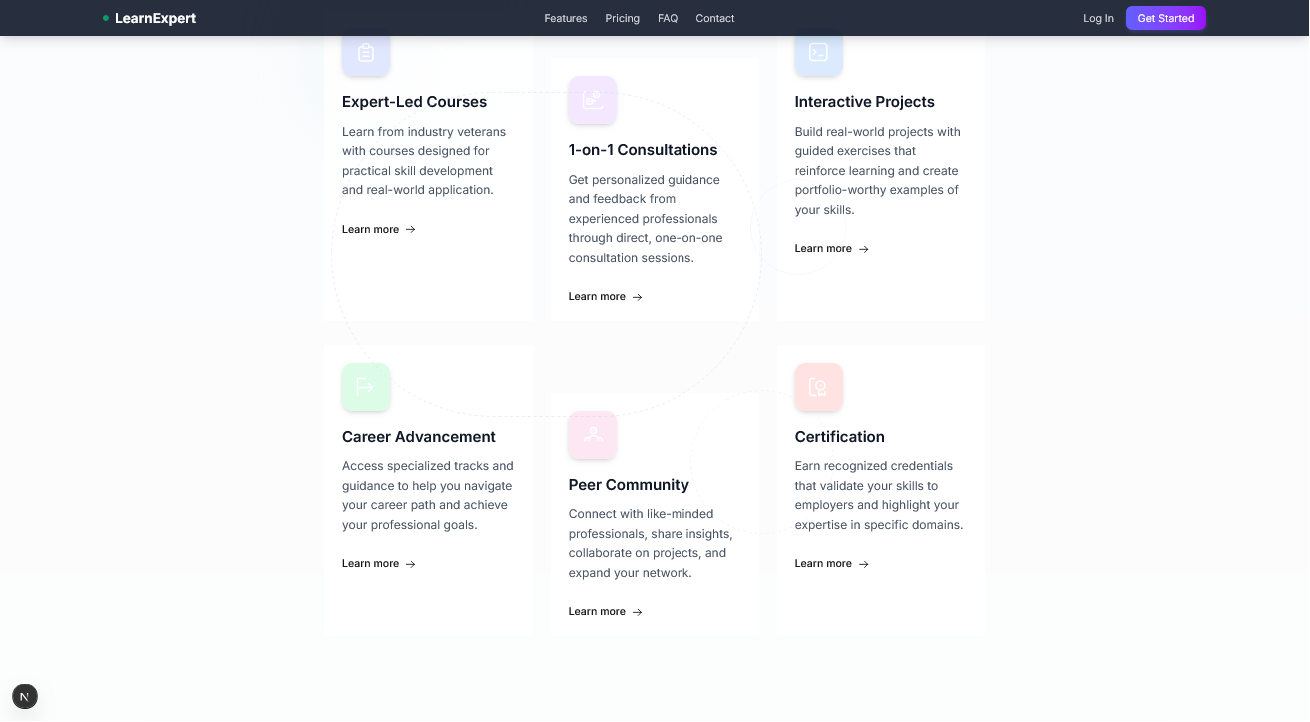
\includegraphics[width=0.9\textwidth,keepaspectratio]{week_2_img/fetchersection_2.png}
  \caption{\textbf{Section de fonctionnalités} présentant les différentes offres de la plateforme.}
  \label{fig:features_section}
\end{figure}

L'approche de développement a été centrée sur :
\begin{itemize}
  \item \textbf{Design responsive :} Adaptation optimale à tous les types d'écrans
  \item \textbf{Animations interactives :} Utilisation de Framer Motion pour des transitions fluides
  \item \textbf{Performance optimisée :} Chargement différé des images et optimisation automatique
  \item \textbf{Accessibilité :} Respect des standards WCAG pour une plateforme inclusive
\end{itemize}

\subsection{Tableau de bord apprenant}

L'interface du tableau de bord apprenant a été développée pendant la semaine 3 pour offrir une expérience personnalisée et intuitive aux utilisateurs connectés.

\begin{figure}[H]
  \centering
  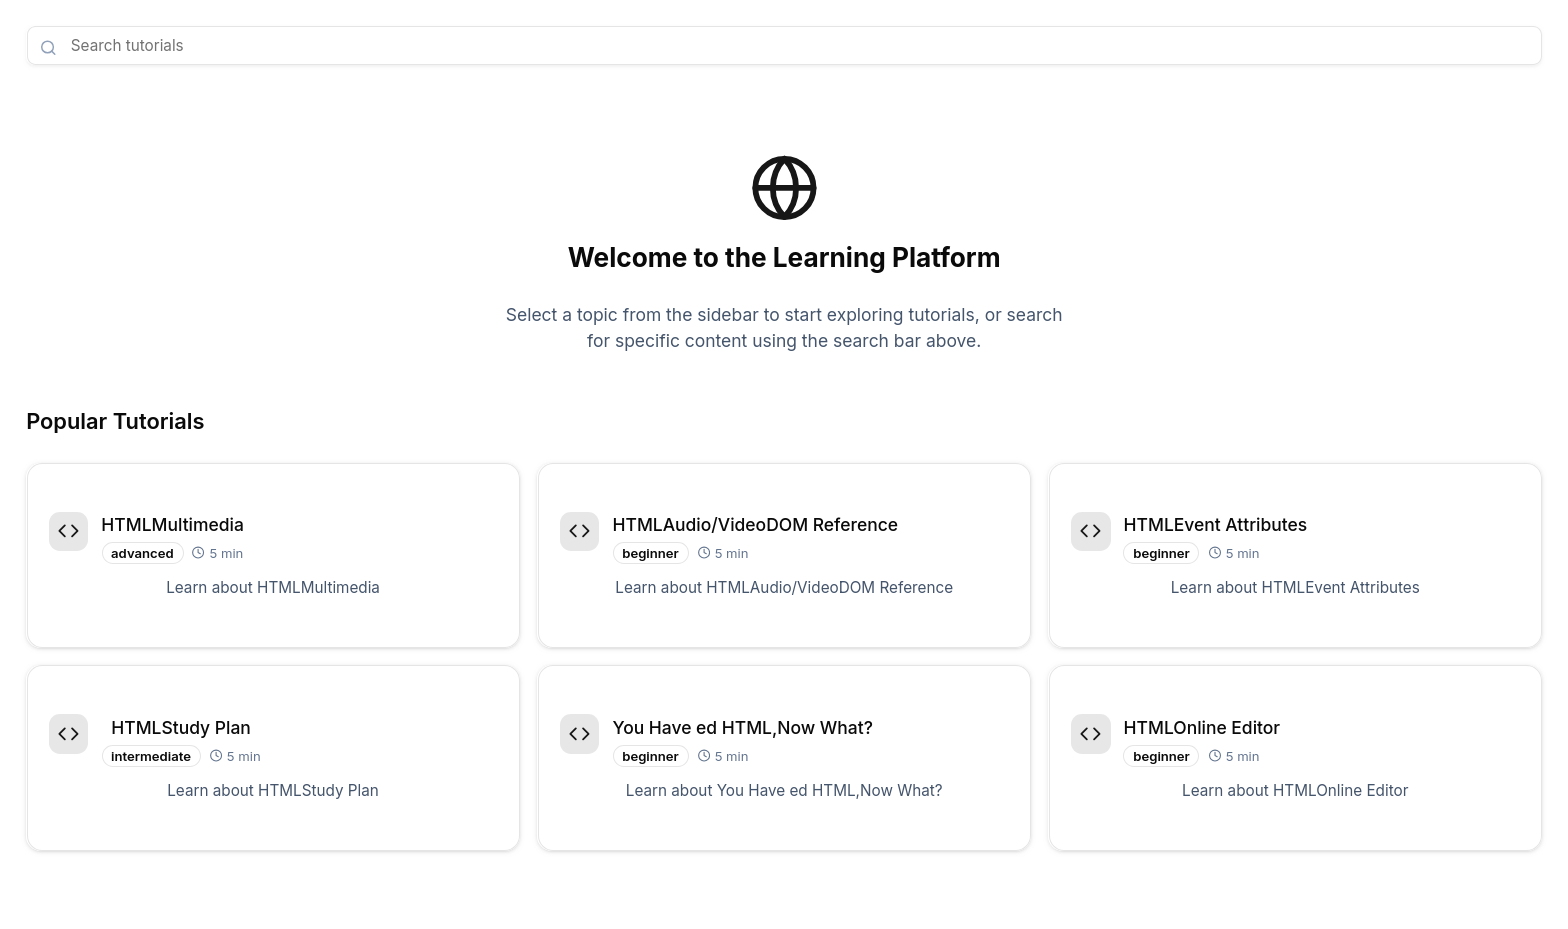
\includegraphics[width=0.9\textwidth,keepaspectratio]{week_3_img/accueil.png}
  \caption{\textbf{Interface d'accueil personnalisée} pour les utilisateurs connectés.}
  \label{fig:dashboard}
\end{figure}

Les principales fonctionnalités implémentées comprennent :
\begin{itemize}
  \item \textbf{Vue d'ensemble des cours en cours :} Affichage des cours commencés avec progression
  \item \textbf{Recommandations personnalisées :} Suggestions de cours basées sur les intérêts et l'historique
  \item \textbf{Dernières activités :} Suivi des activités récentes de l'utilisateur
  \item \textbf{Notifications :} Alertes pour les mises à jour de cours et échéances
\end{itemize}

Une attention particulière a été portée à l'ergonomie de l'interface, avec une barre latérale de navigation intuitive permettant d'accéder facilement aux différentes sections de la plateforme.

\begin{figure}[H]
  \centering
  
\includegraphics[width=0.4\textwidth,keepaspectratio]{week_3_img/sidebare.png}
  \caption{\textbf{Barre latérale de navigation} avec accès aux principales fonctionnalités.}
  \label{fig:sidebar}
\end{figure}

\subsection{Interface de consultation des cours}

L'interface de consultation des cours a été conçue pour offrir une expérience d'apprentissage immersive et efficace, avec une organisation claire du contenu théorique et pratique.

\begin{figure}[H]
  \centering
  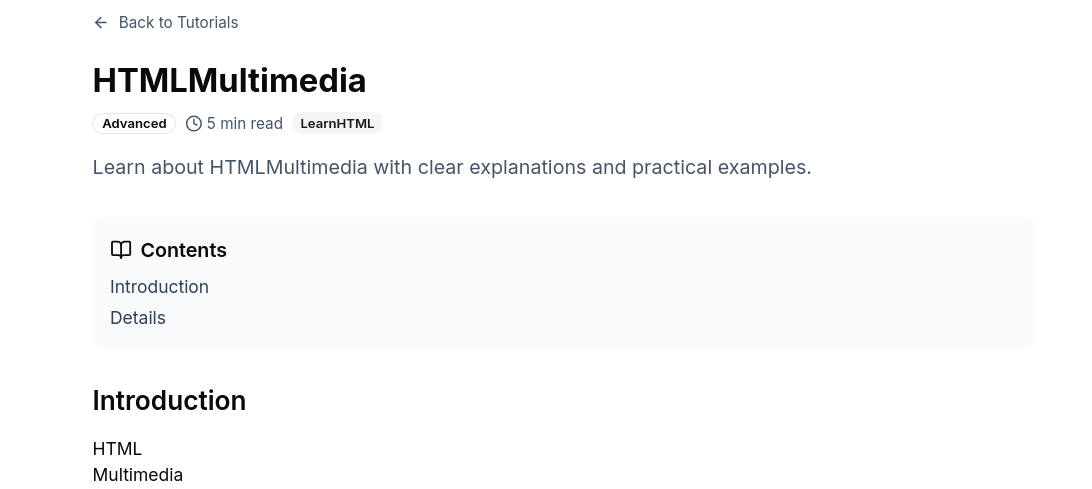
\includegraphics[width=0.9\textwidth,keepaspectratio]{week_3_img/part1.png}
  \caption{\textbf{Interface de consultation des cours} - Partie théorique.}
  \label{fig:course_theory}
\end{figure}

\begin{figure}[H]
  \centering
  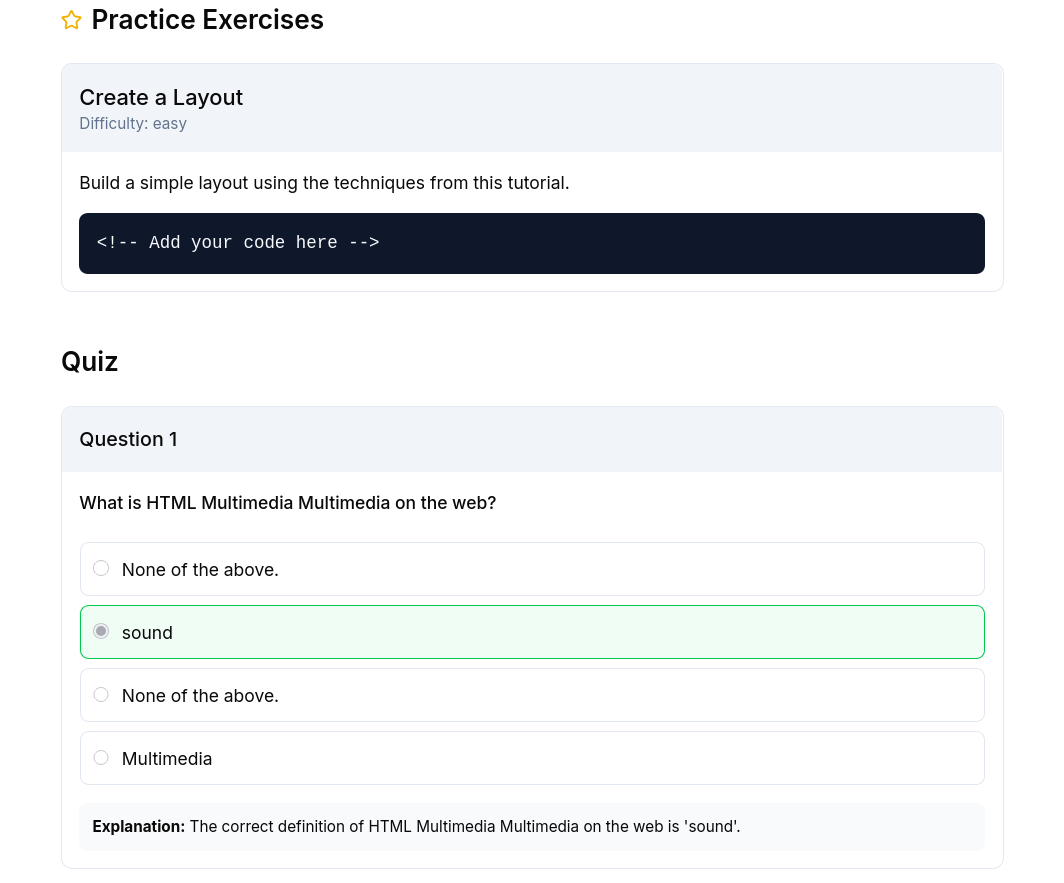
\includegraphics[width=0.9\textwidth,keepaspectratio]{week_3_img/part2.png}
  \caption{\textbf{Interface de consultation des cours} - Partie pratique avec exercices interactifs.}
  \label{fig:course_practice}
\end{figure}

Les fonctionnalités clés de cette interface incluent :
\begin{itemize}
  \item \textbf{Contenu structuré :} Organisation claire avec sections théoriques et pratiques
  \item \textbf{Éditeur de code interactif :} Basé sur Monaco Editor pour tester le code en temps réel
  \item \textbf{Exercices intégrés :} Pratique directement dans l'interface avec feedback immédiat
  \item \textbf{Suivi de progression :} Visualisation claire de l'avancement dans le cours
  \item \textbf{Mode sombre/clair :} Adaptation de l'interface aux préférences de l'utilisateur
  \item \textbf{Plan du cours :} Navigation facile entre les différentes sections
\end{itemize}

\subsection{Améliorations UI/UX avancées}

Durant la quatrième semaine, d'importantes améliorations ont été apportées à l'expérience utilisateur pour rendre la plateforme plus intuitive et engageante.

\subsubsection{Interactivité des exemples de code}

Une refonte significative de la section des exemples de code a été entreprise pour la rendre entièrement interactive :
\begin{itemize}
    \item \textbf{Coloration syntaxique avancée :} Implémentation d'une coloration syntaxique précise pour plus de 6 langages de programmation (JavaScript, Python, HTML, CSS, C/C++)
    \item \textbf{Édition directe :} Possibilité pour les utilisateurs de modifier le code et de voir les résultats en temps réel
    \item \textbf{Prévisualisation instantanée :} Visualisation immédiate du rendu pour les langages web (HTML, CSS, JavaScript)
    \item \textbf{Modes d'affichage flexibles :} Options pour changer la disposition (verticale, horizontale, ou écran partagé)
    \item \textbf{Mode plein écran :} Option pour agrandir l'éditeur et se concentrer sur le code
    \item \textbf{Personnalisation des thèmes :} Possibilité de choisir entre différents thèmes d'édition (clair, sombre, GitHub, Monokai)
\end{itemize}

\begin{figure}[H]
  \centering
  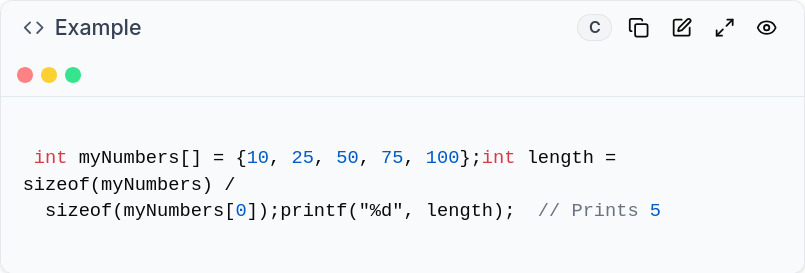
\includegraphics[width=0.4\textwidth,keepaspectratio]{old-reports/week_4_img/pre_edit.jpeg}
  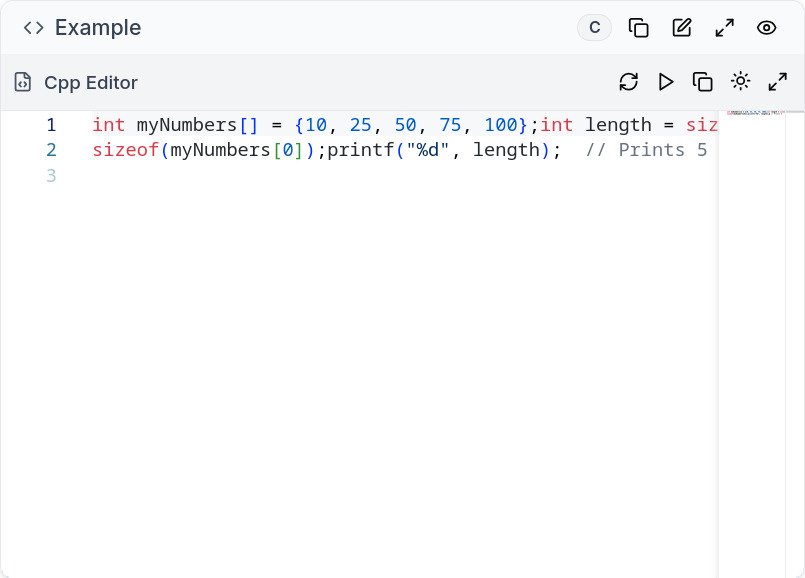
\includegraphics[width=0.4\textwidth,keepaspectratio]{old-reports/week_4_img/editmode.jpeg}
  \caption{\textbf{Éditeur de code interactif} avec options d'édition et coloration syntaxique.}
  \label{fig:code_editor}
\end{figure}

\begin{figure}[H]
  \centering
  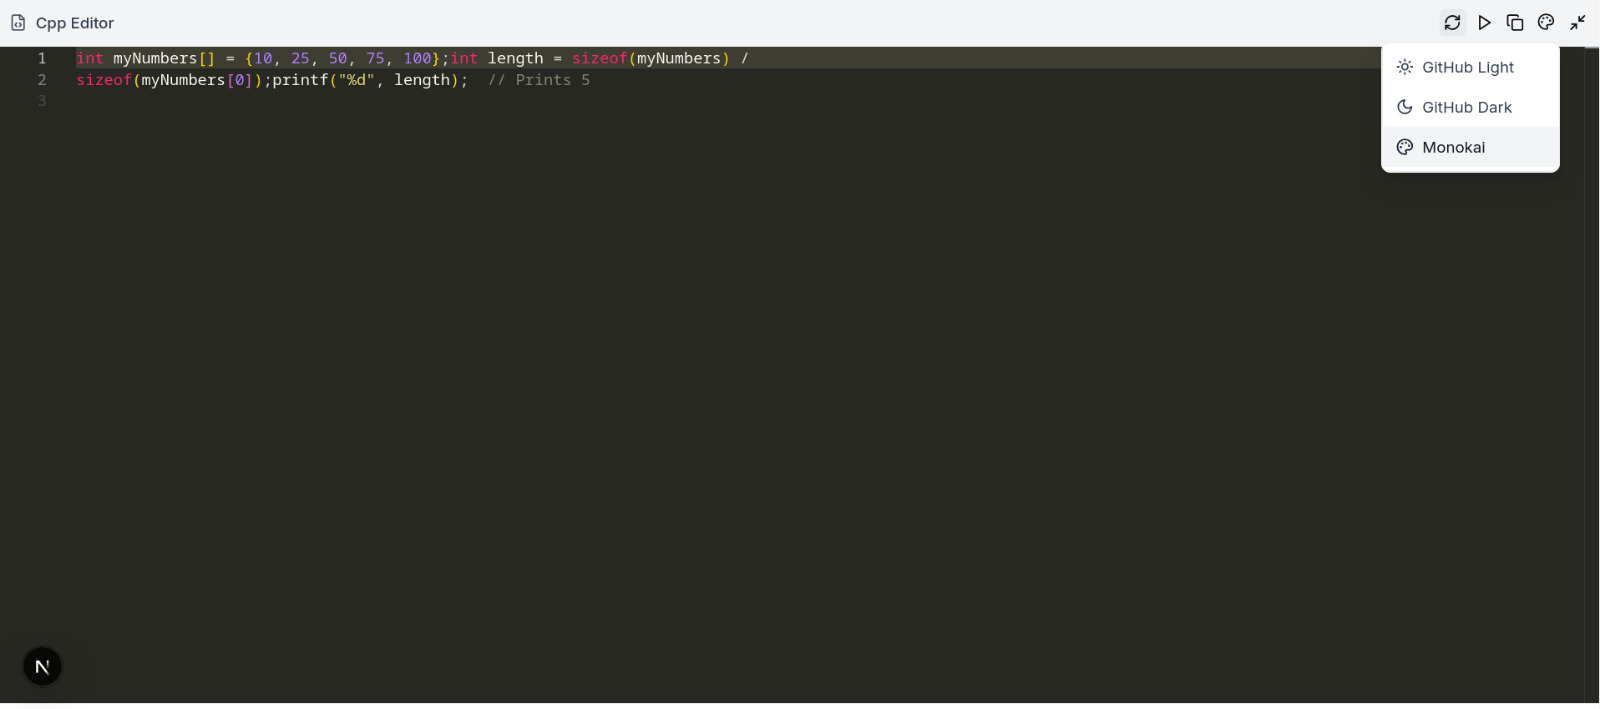
\includegraphics[width=0.5\textwidth,keepaspectratio]{old-reports/week_4_img/expended.jpeg}
  \caption{\textbf{Mode plein écran} de l'éditeur de code avec thème personnalisé.}
  \label{fig:code_editor_fullscreen}
\end{figure}

\subsubsection{Navigation et structure améliorées}

Pour faciliter l'accès au contenu et améliorer l'expérience globale d'apprentissage :
\begin{itemize}
    \item \textbf{Plan du cours interactif :} Implémentation d'une structure claire des modules et leçons permettant une navigation directe
    \item \textbf{Mode focus dans la barre latérale :} Possibilité de masquer les catégories non pertinentes pour se concentrer sur le cours actuel
    \item \textbf{Indicateurs de progression visuels :} Affichage clair de l'avancement dans chaque section du cours
\end{itemize}

\begin{figure}[H]
  \centering
  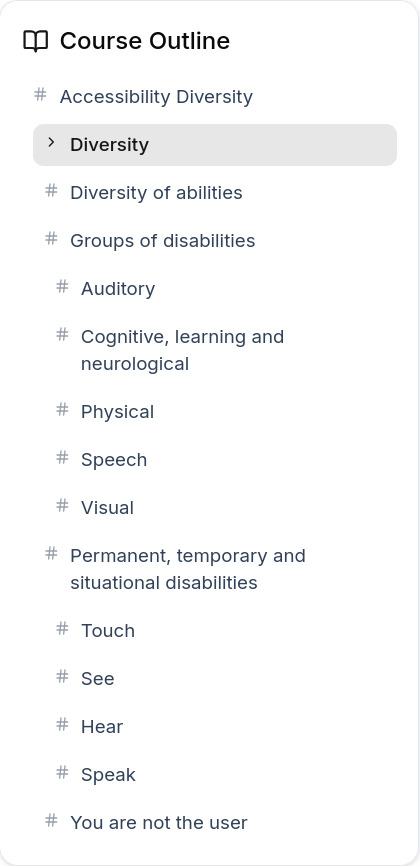
\includegraphics[width=0.4\textwidth,keepaspectratio]{old-reports/week_4_img/outline.jpeg}
  
\includegraphics[width=0.4\textwidth,keepaspectratio]{old-reports/week_4_img/sidebare2.jpeg}
  \caption{\textbf{Plan du cours et barre latérale améliorée} avec focus sur la section active.}
  \label{fig:navigation_improved}
\end{figure}

\subsection{Interfaces utilisateur premium}

Un ensemble complet d'interfaces pour les utilisateurs premium a été développé afin de fournir une expérience enrichie :

\begin{itemize}
    \item \textbf{Tableau de bord premium :} Vue d'ensemble personnalisée avec statistiques avancées et suivi détaillé de la progression
    \item \textbf{Page des paramètres utilisateur :} Interface complète pour gérer le profil, les préférences de notification et les paramètres de sécurité
    \item \textbf{Page d'exploration des cours :} Catalogue interactif avec options de filtrage et de recherche avancées
    \item \textbf{Forums et communauté :} Espace dédié aux discussions et au partage de connaissances entre apprenants
    \item \textbf{Parcours d'apprentissage personnalisés :} Séquences de cours structurées adaptées aux objectifs de carrière spécifiques
\end{itemize}

\begin{figure}[H]
  \centering
  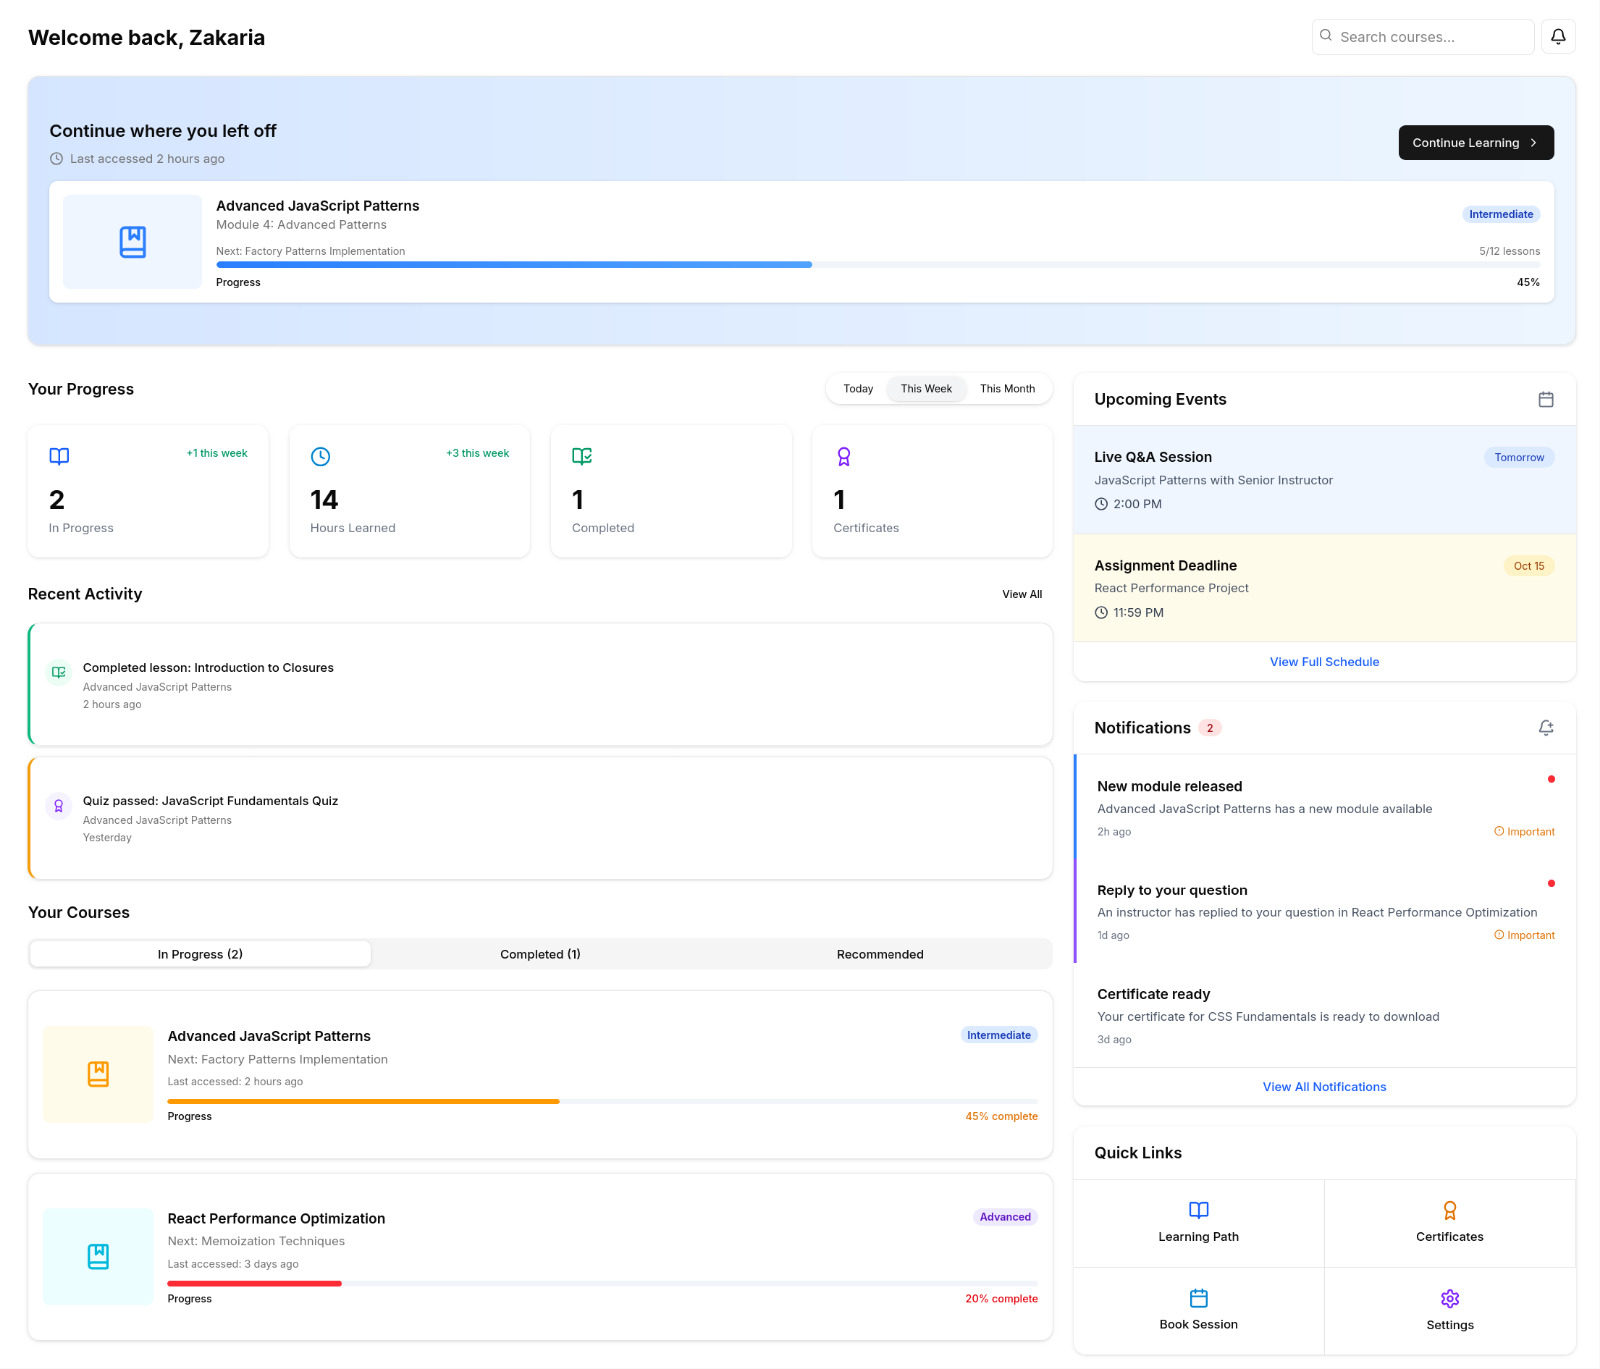
\includegraphics[width=0.85\textwidth,keepaspectratio]{old-reports/week_4_img/dashboard.jpeg}
  \caption{\textbf{Tableau de bord premium} avec statistiques détaillées et recommandations personnalisées.}
  \label{fig:premium_dashboard}
\end{figure}

\begin{figure}[H]
  \centering
  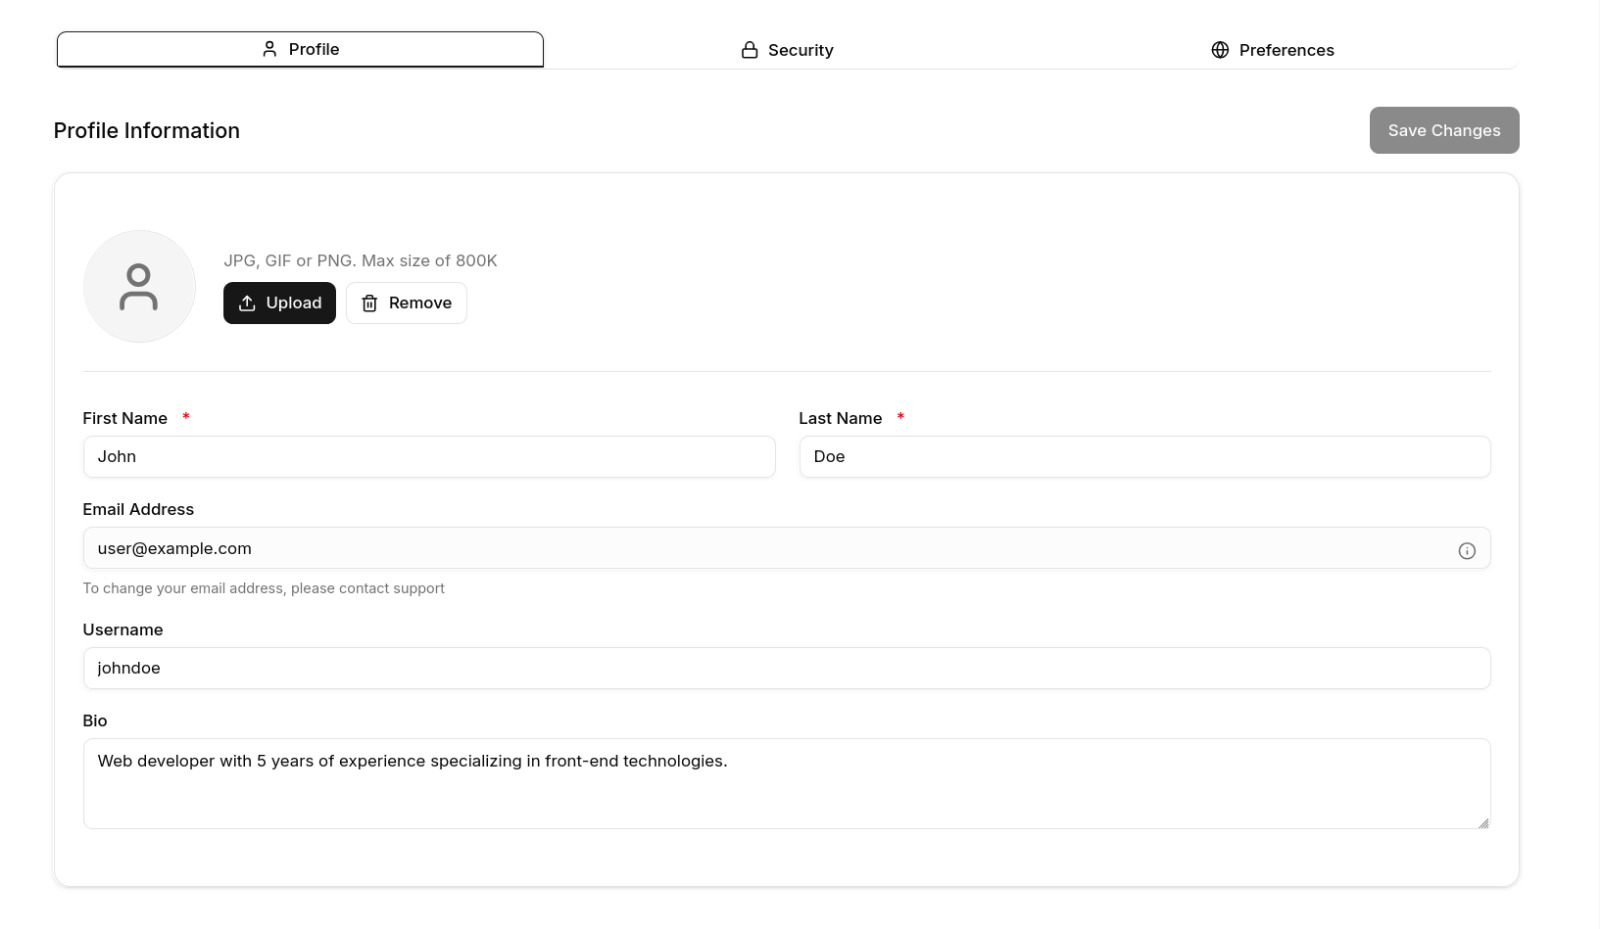
\includegraphics[width=0.85\textwidth,keepaspectratio]{old-reports/week_4_img/settings.jpeg}
  \caption{\textbf{Page des paramètres utilisateur} avec options de personnalisation avancées.}
  \label{fig:user_settings}
\end{figure}

\begin{figure}[H]
  \centering
  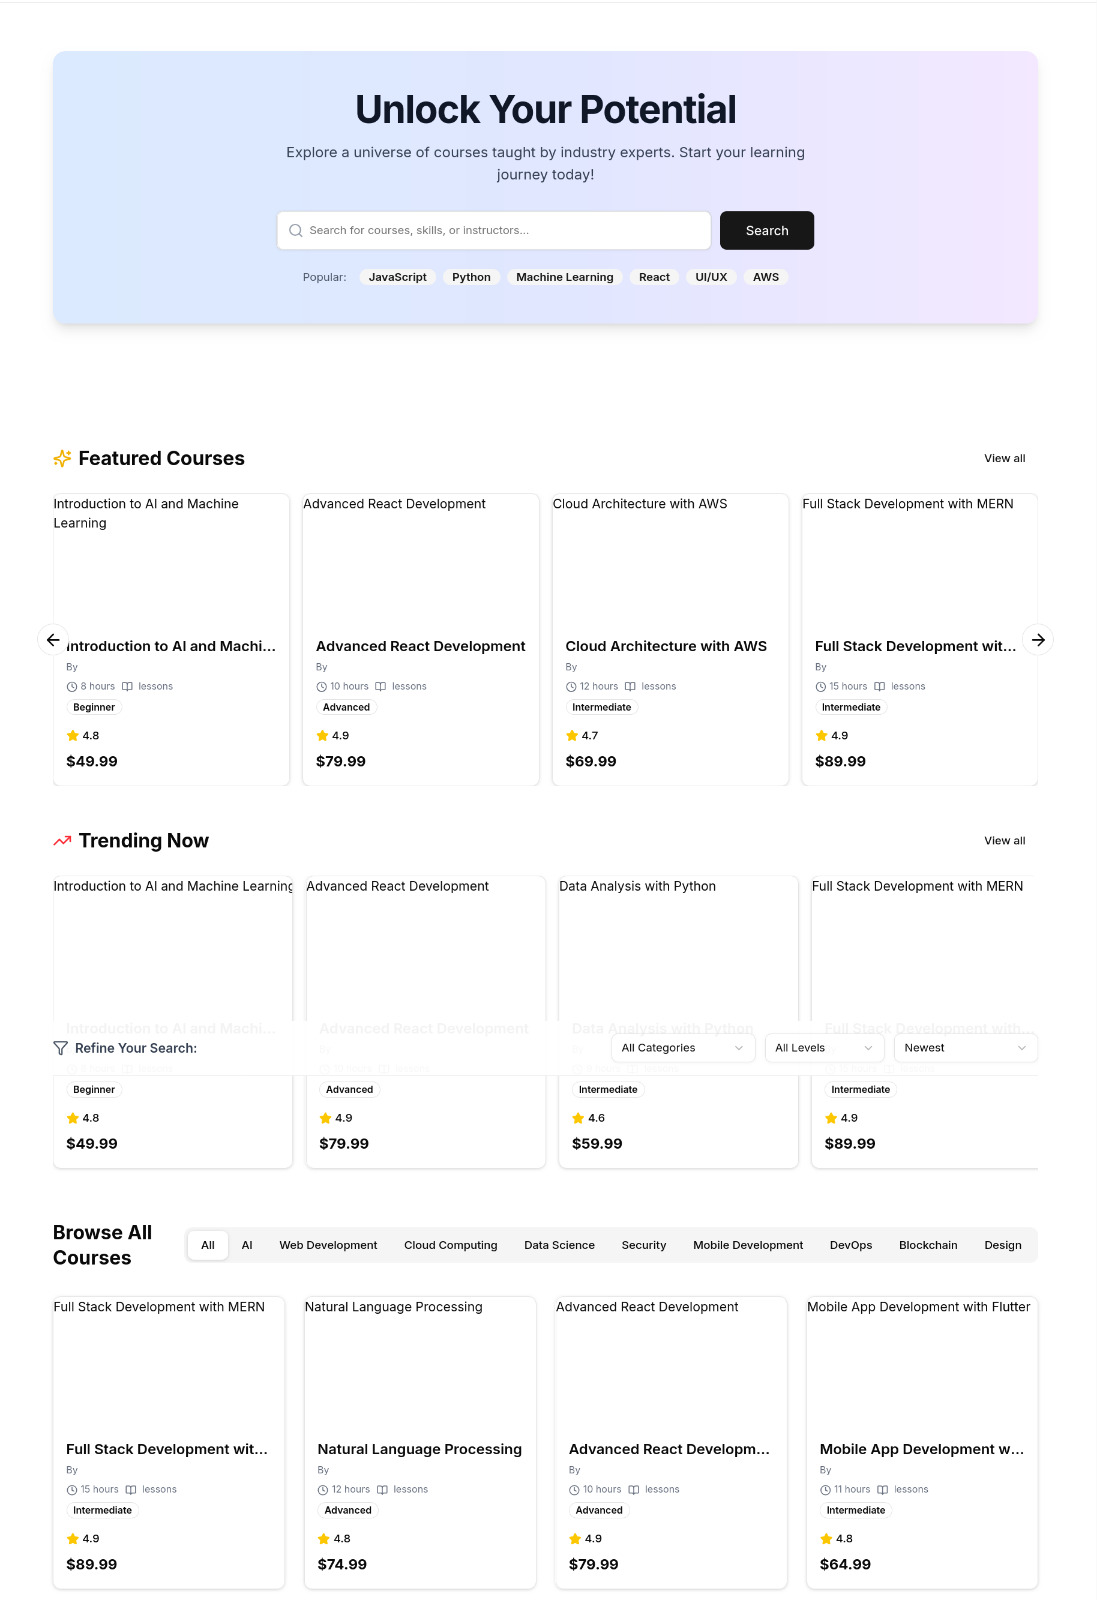
\includegraphics[width=0.85\textwidth,keepaspectratio]{old-reports/week_4_img/explor.jpeg}
  \caption{\textbf{Page d'exploration des cours} avec filtres avancés et suggestions personnalisées.}
  \label{fig:course_explorer}
\end{figure}

\begin{figure}[H]
  \centering
  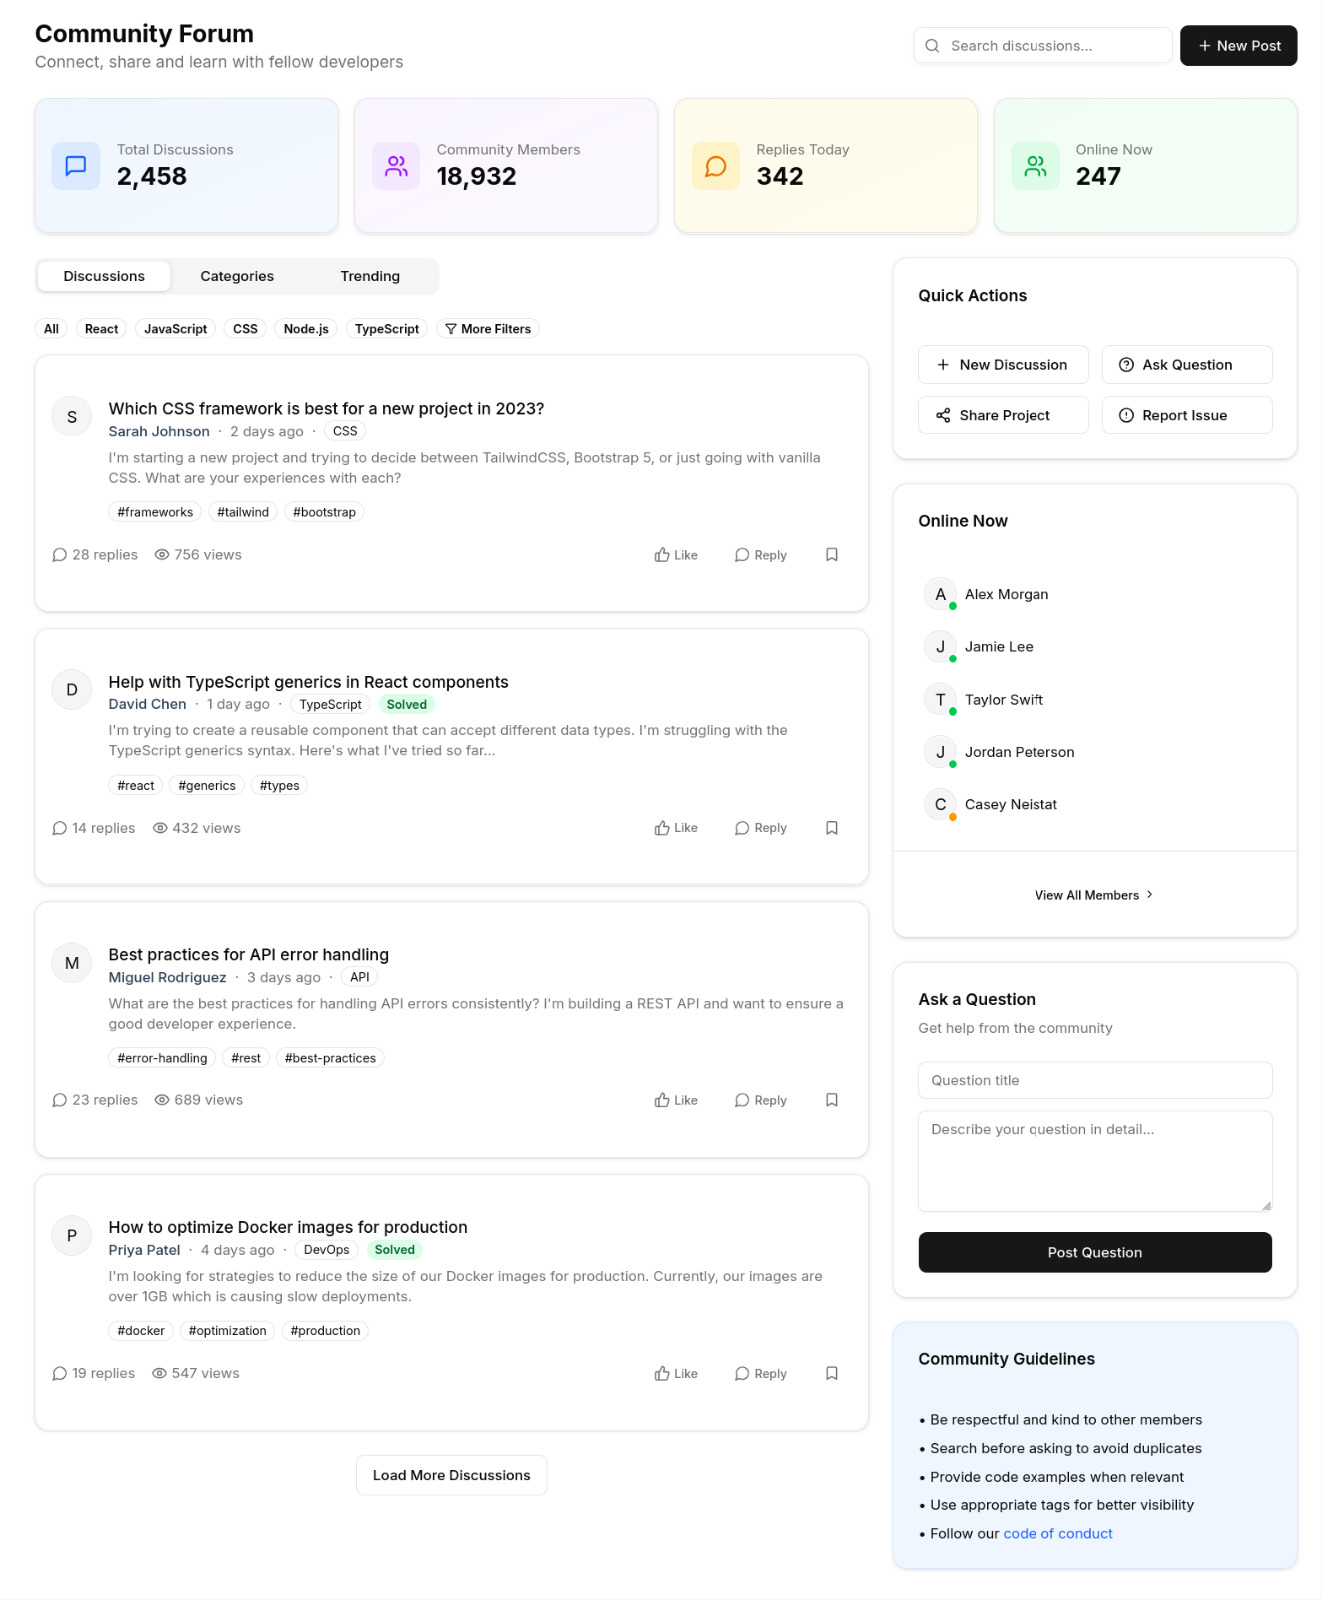
\includegraphics[width=0.85\textwidth,keepaspectratio]{old-reports/week_4_img/froms.jpeg}
  \caption{\textbf{Forums de discussion} pour l'échange entre apprenants et formateurs.}
  \label{fig:community_forums}
\end{figure}

\begin{figure}[H]
  \centering
  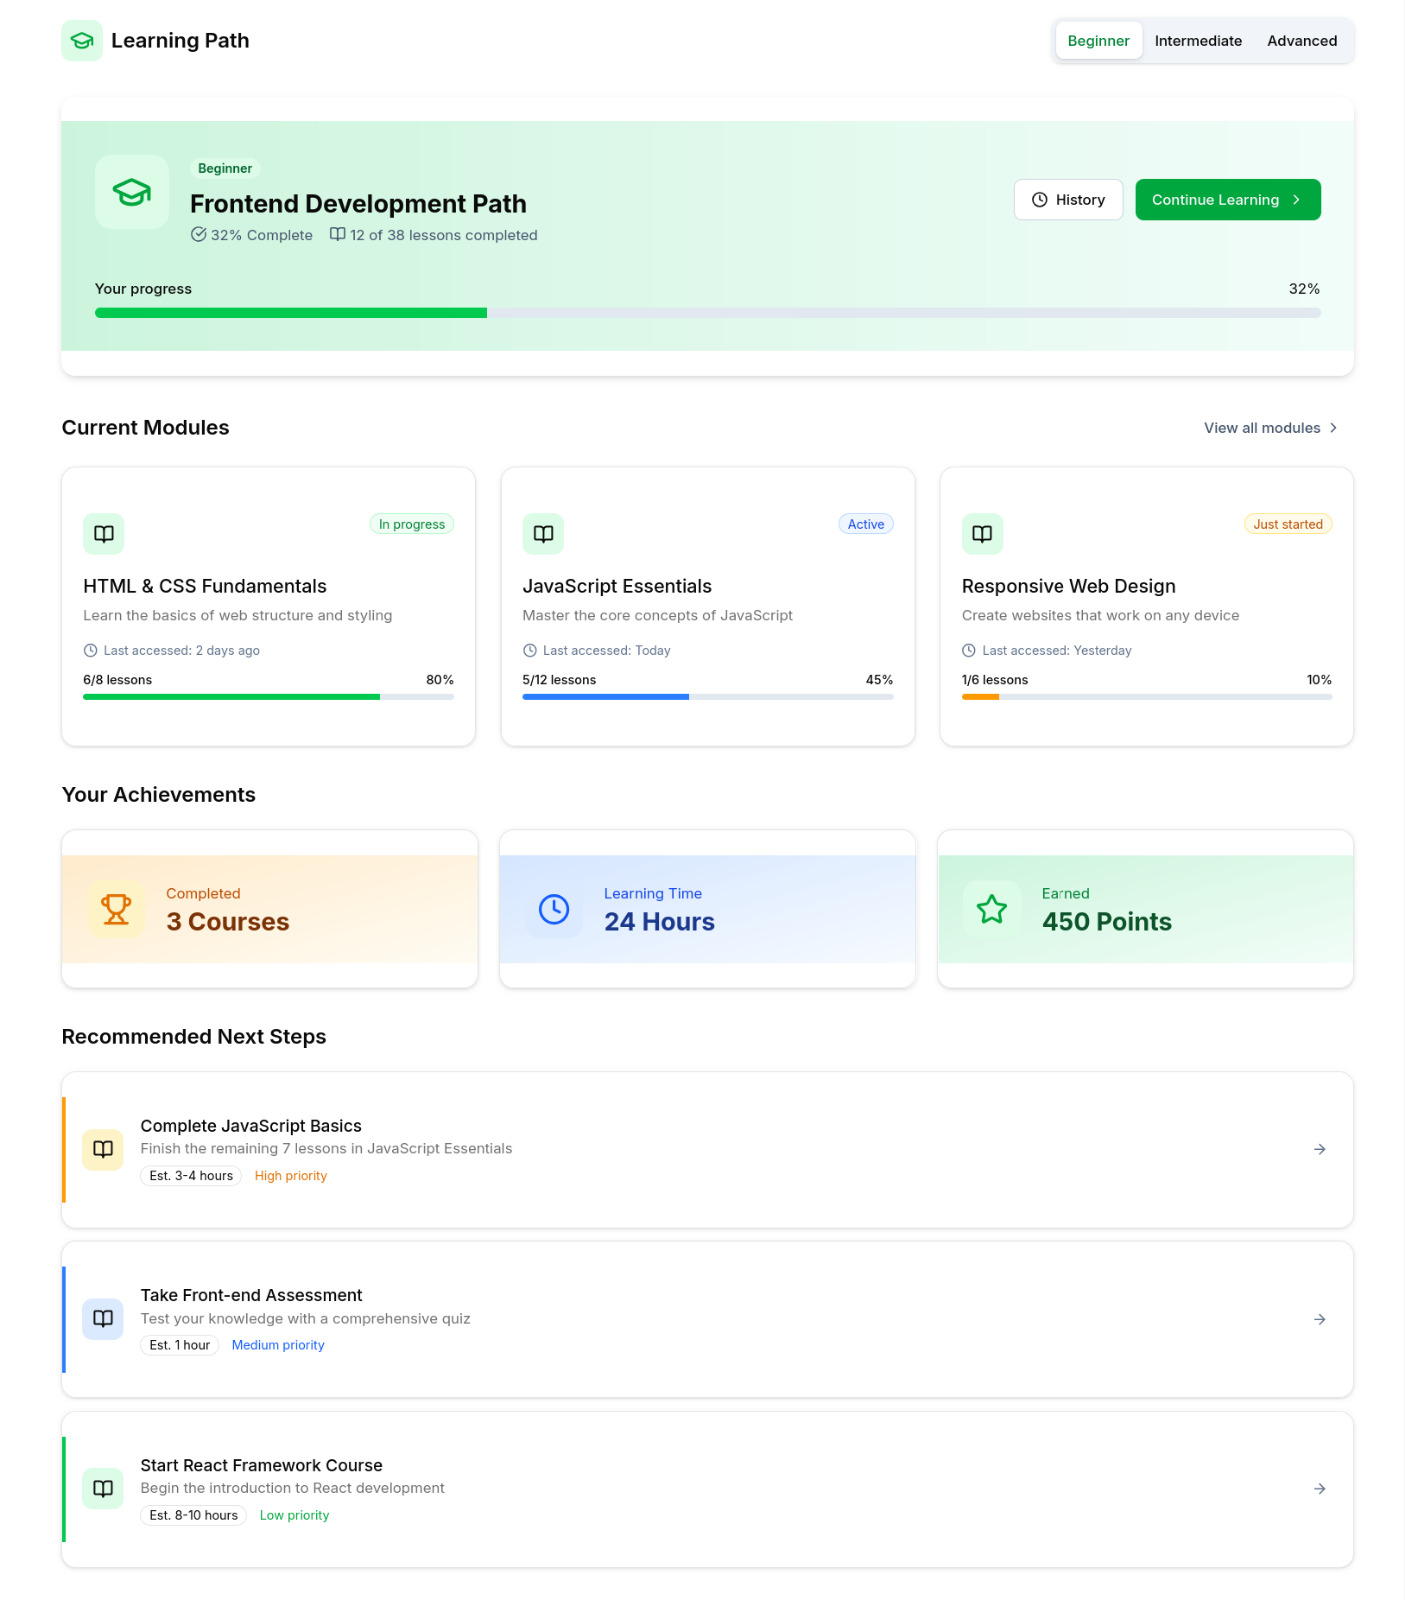
\includegraphics[width=0.85\textwidth,keepaspectratio]{old-reports/week_4_img/learnpath.jpeg}
  \caption{\textbf{Parcours d'apprentissage personnalisé} avec progression structurée.}
  \label{fig:learning_paths}
\end{figure}

\subsection{Interfaces d'administration et de gestion}

Une partie significative du développement a été consacrée à la création d'interfaces d'administration complètes pour la gestion de la plateforme :

\begin{itemize}
  \item \textbf{Tableau de bord administrateur :} Vue centralisée avec statistiques globales et accès à toutes les fonctionnalités d'administration
  \item \textbf{Gestion des utilisateurs :} Interface pour créer, modifier et gérer les comptes utilisateurs avec contrôle des rôles et permissions
  \item \textbf{Gestion des cours :} Outils pour créer, éditer et organiser le contenu des cours
  \item \textbf{Modération de contenu :} Interface pour examiner et approuver les contributions des utilisateurs
  \item \textbf{Analyse et rapports :} Tableaux de bord analytiques pour suivre l'engagement et les performances des utilisateurs
  \item \textbf{Gestion des abonnements :} Outils pour gérer les plans d'abonnement et les paiements
\end{itemize}

\begin{figure}[H]
  \centering
  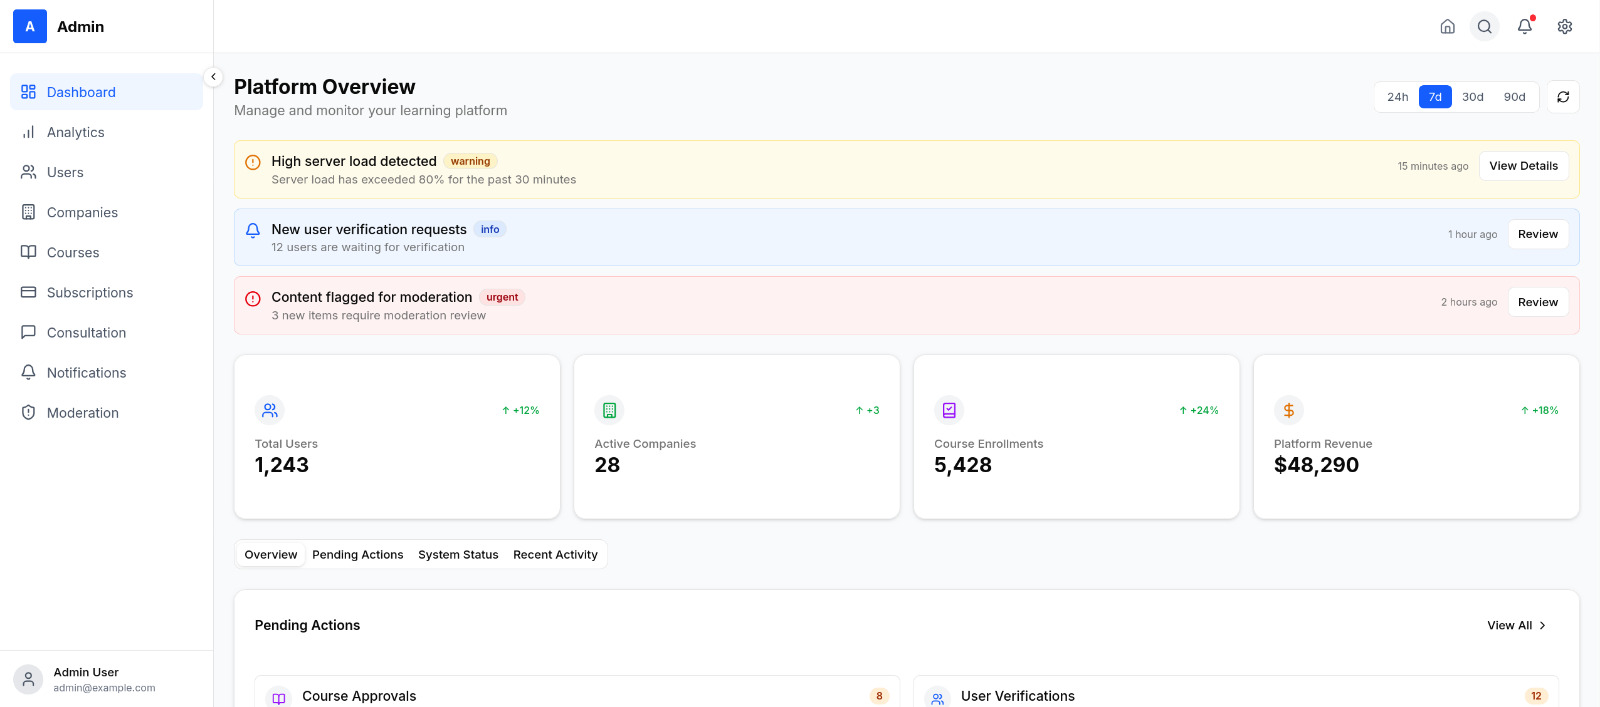
\includegraphics[width=0.85\textwidth,keepaspectratio]{old-reports/week_4_img/admin.jpeg}
  \caption{\textbf{Tableau de bord administrateur} avec vue d'ensemble des métriques de la plateforme.}
  \label{fig:admin_dashboard}
\end{figure}

\begin{figure}[H]
  \centering
  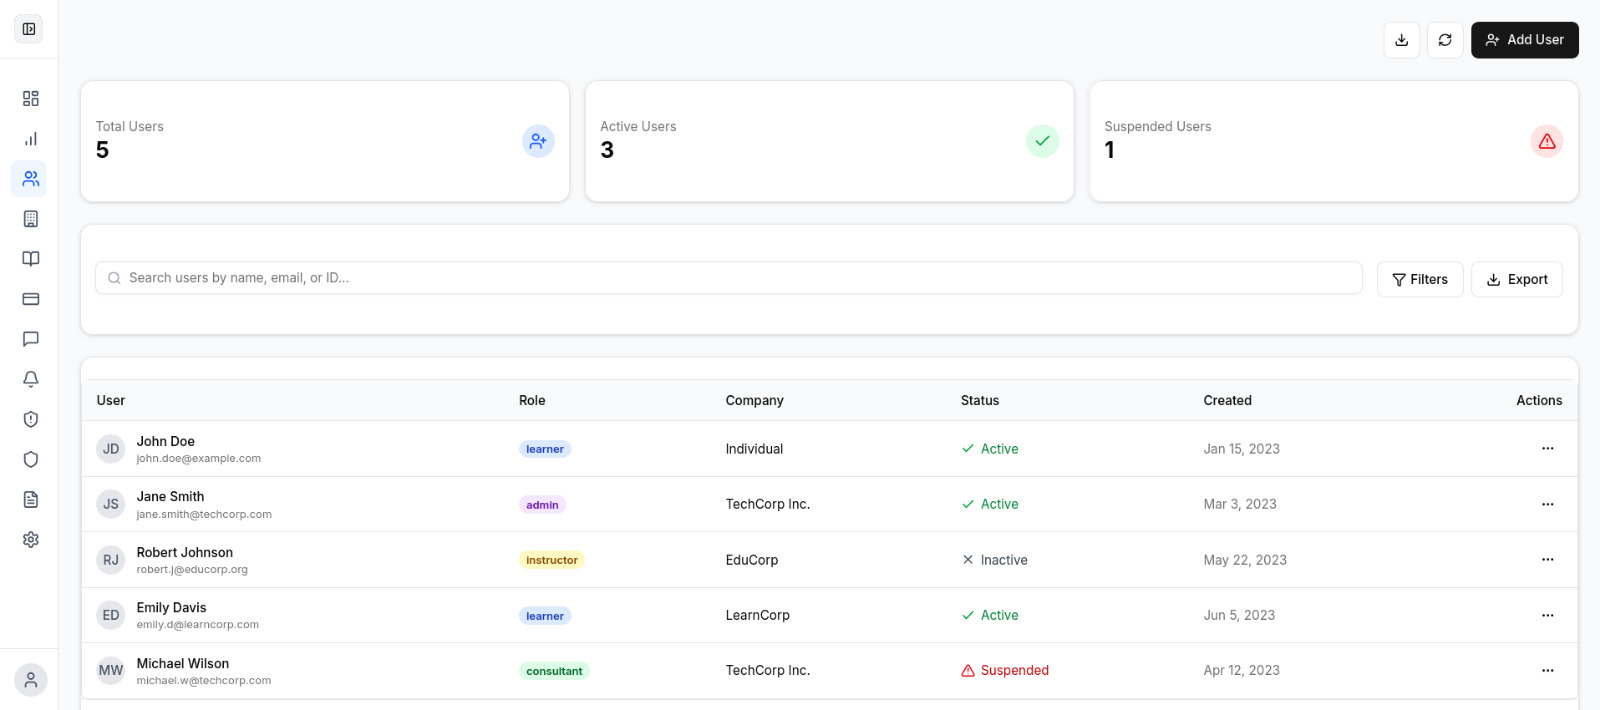
\includegraphics[width=0.85\textwidth,keepaspectratio]{old-reports/week_4_img/usrmana.jpeg}
  \caption{\textbf{Interface de gestion des utilisateurs} pour l'administration des comptes.}
  \label{fig:user_management}
\end{figure}

\begin{figure}[H]
  \centering
  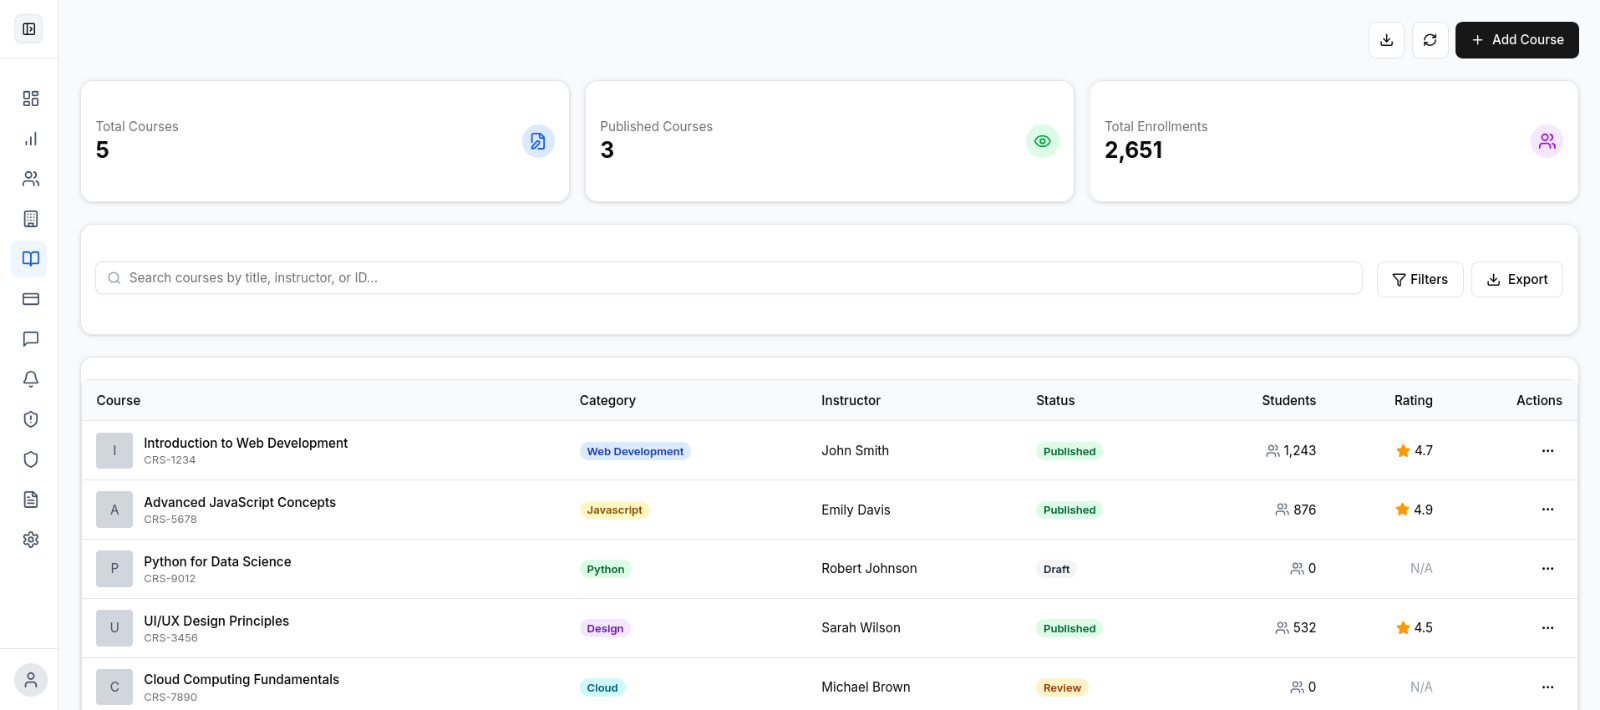
\includegraphics[width=0.85\textwidth,keepaspectratio]{old-reports/week_4_img/coursmanagement.jpeg}
  \caption{\textbf{Interface de gestion des cours} permettant l'organisation du contenu éducatif.}
  \label{fig:course_management}
\end{figure}

\begin{figure}[H]
  \centering
  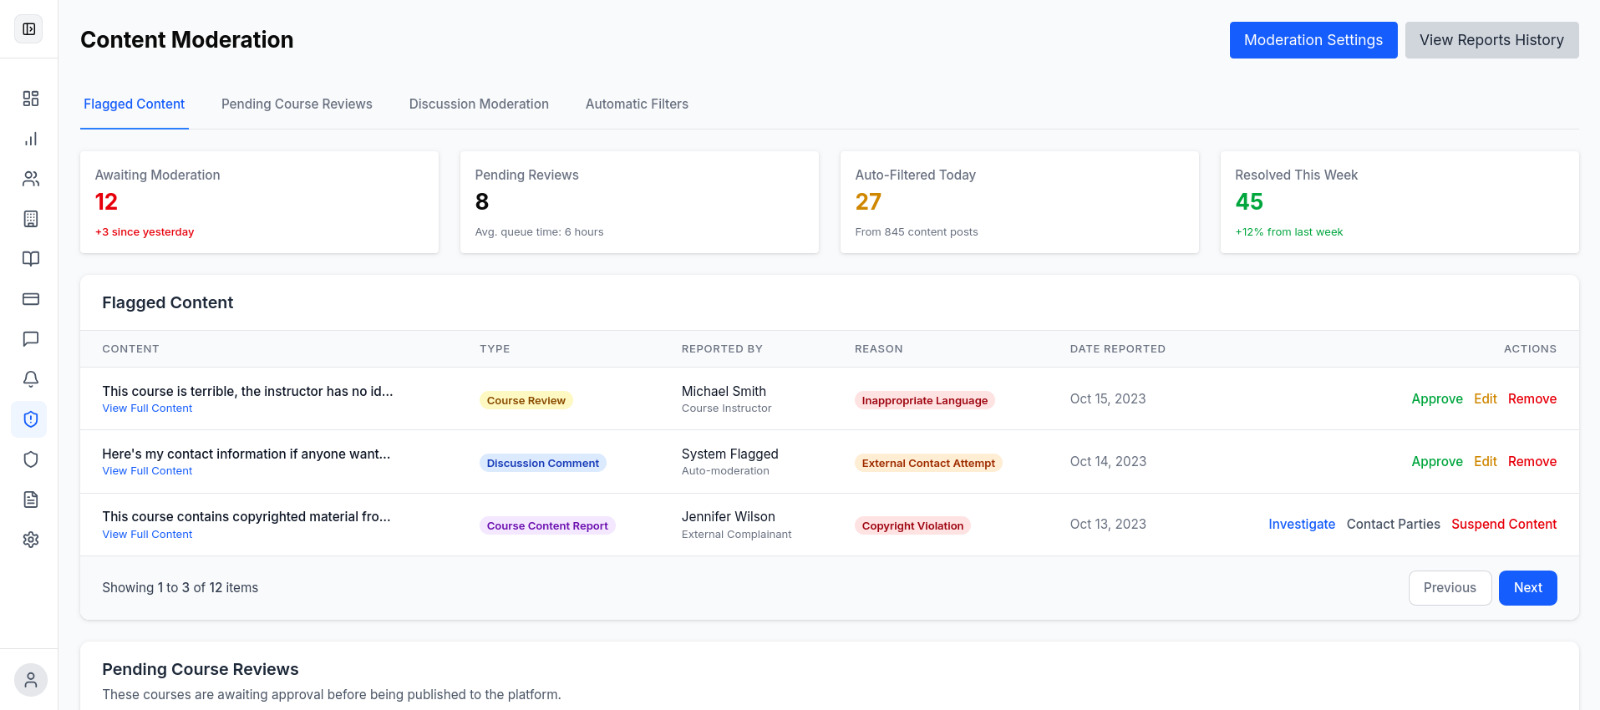
\includegraphics[width=0.85\textwidth,keepaspectratio]{old-reports/week_4_img/contentmod.jpeg}
  \caption{\textbf{Interface de modération de contenu} pour maintenir la qualité des ressources.}
  \label{fig:content_moderation}
\end{figure}

\begin{figure}[H]
  \centering
  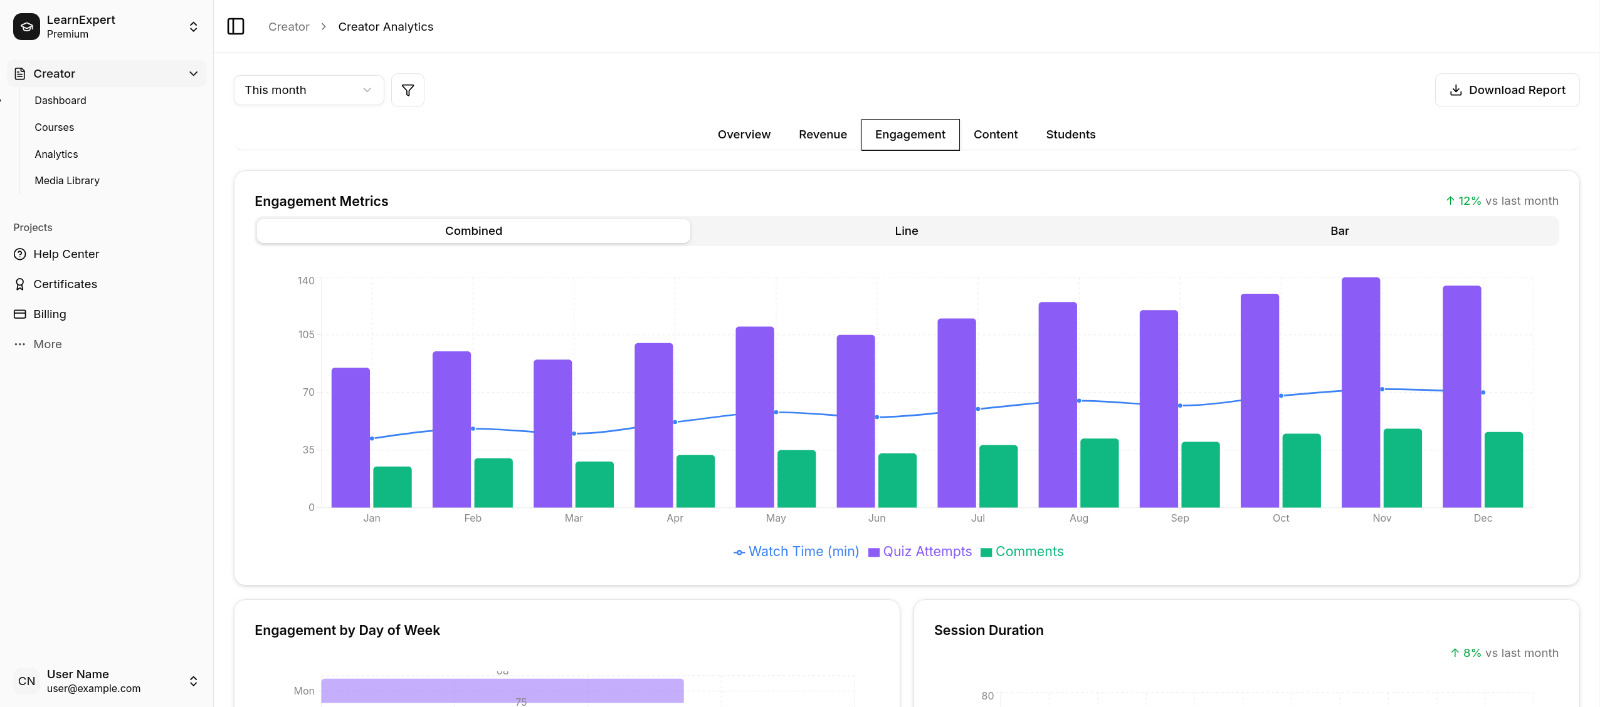
\includegraphics[width=0.85\textwidth,keepaspectratio]{old-reports/week_4_img/analytics.jpeg}
  \caption{\textbf{Tableaux de bord analytiques} pour suivre les performances de la plateforme.}
  \label{fig:analytics_dashboard}
\end{figure}

\begin{figure}[H]
  \centering
  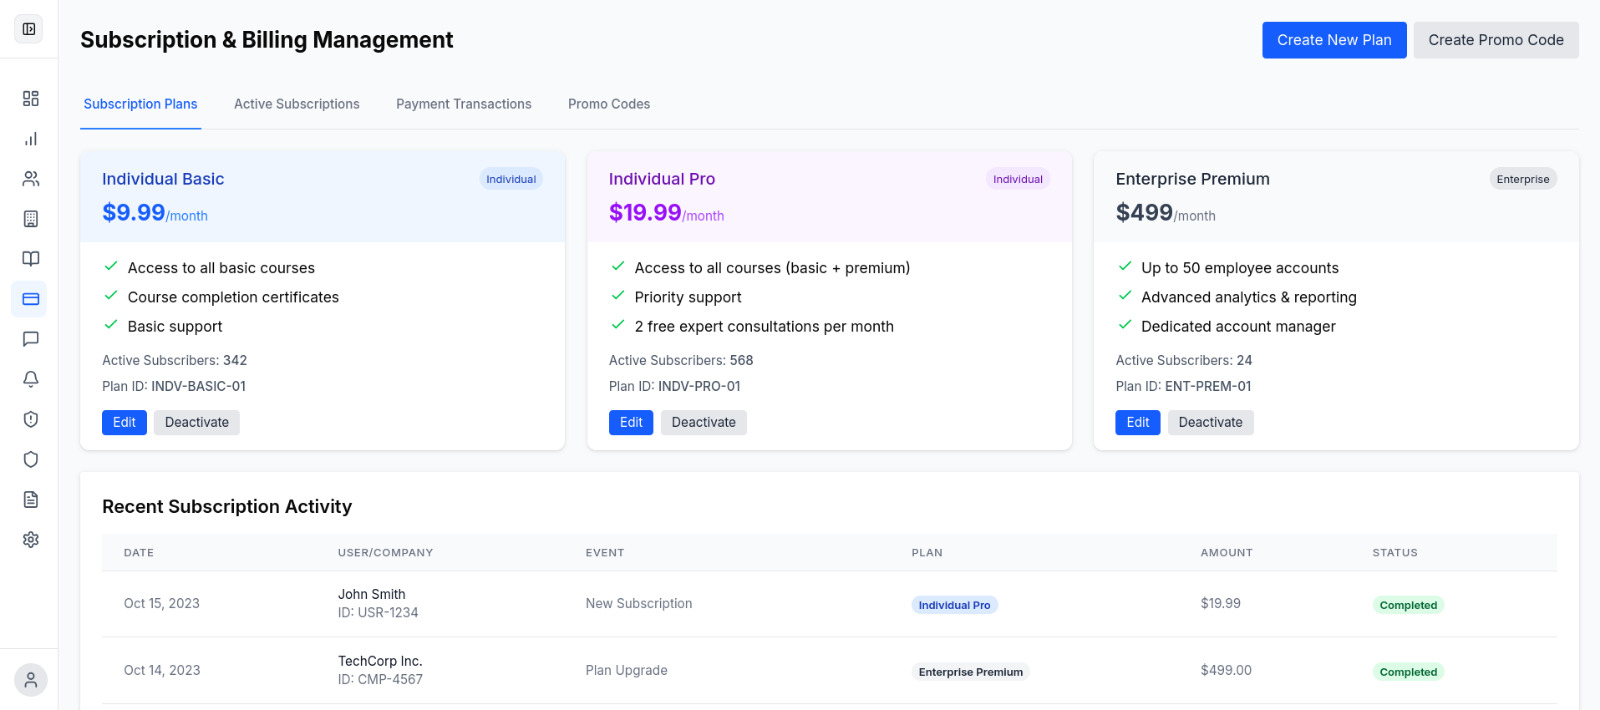
\includegraphics[width=0.85\textwidth,keepaspectratio]{old-reports/week_4_img/sub.jpeg}
  \caption{\textbf{Gestion des abonnements} pour administrer les plans et paiements.}
  \label{fig:subscription_management}
\end{figure}

\subsection{Système d'authentification et sécurité}

Un système d'authentification robuste a été implémenté pour garantir la sécurité des utilisateurs et de leurs données :

\begin{itemize}
  \item \textbf{Inscription et connexion sécurisées :} Formulaires avec validation avancée et protection contre les attaques courantes
  \item \textbf{Récupération de mot de passe :} Processus de réinitialisation sécurisé avec confirmation par email
  \item \textbf{Journalisation des activités :} Suivi et audit des actions des utilisateurs pour détecter les comportements suspects
  \item \textbf{Gestion des sessions :} Contrôle des sessions actives avec possibilité de révocation
\end{itemize}

\begin{figure}[H]
  \centering
  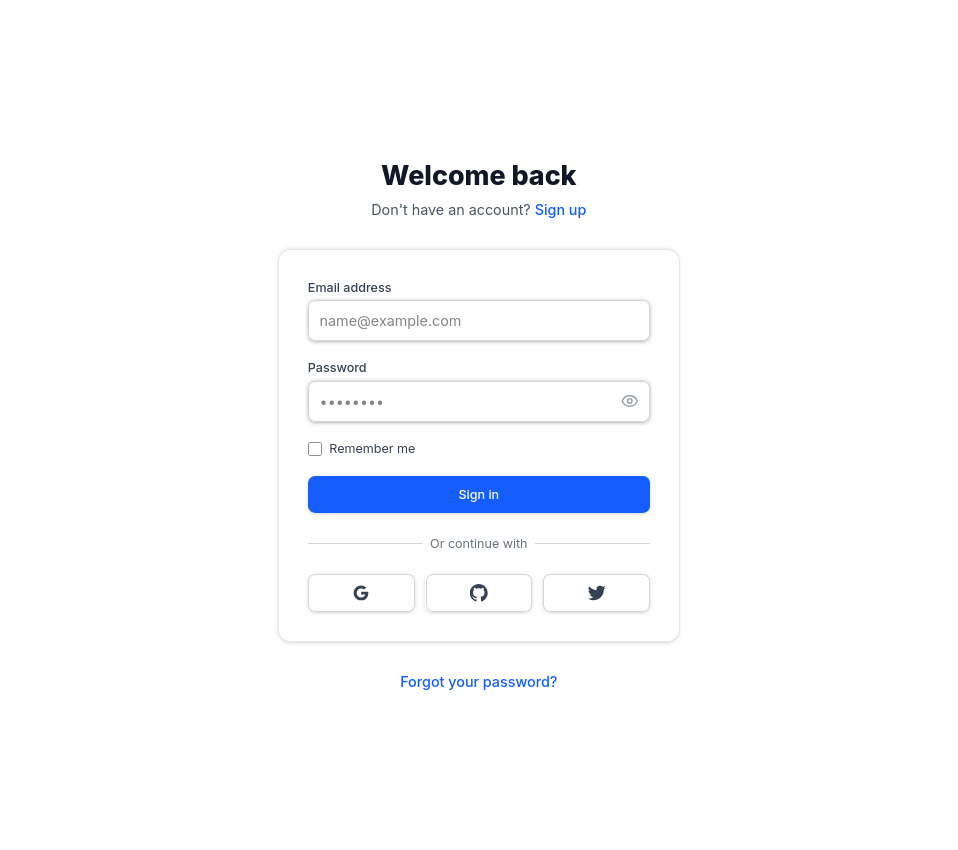
\includegraphics[width=0.4\textwidth,keepaspectratio]{old-reports/week_4_img/login.jpeg}
  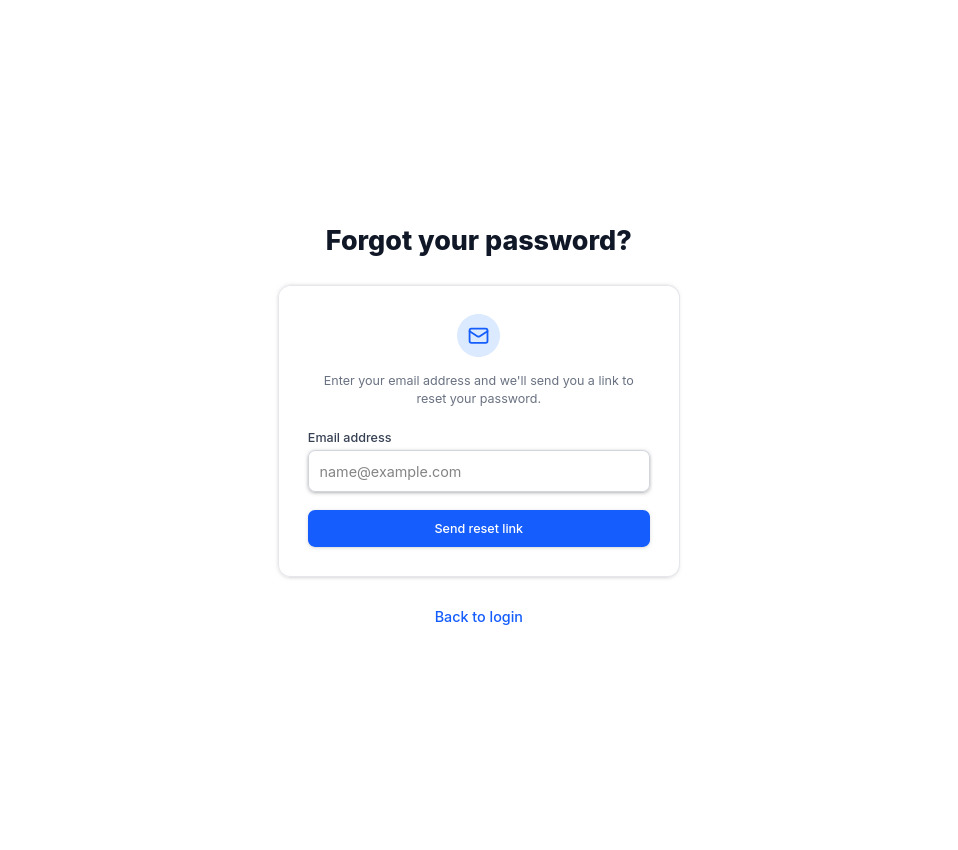
\includegraphics[width=0.4\textwidth,keepaspectratio]{old-reports/week_4_img/reset.jpeg}
  \caption{\textbf{Interfaces de connexion et de réinitialisation de mot de passe} sécurisées.}
  \label{fig:auth_interfaces}
\end{figure}

\begin{figure}[H]
  \centering
  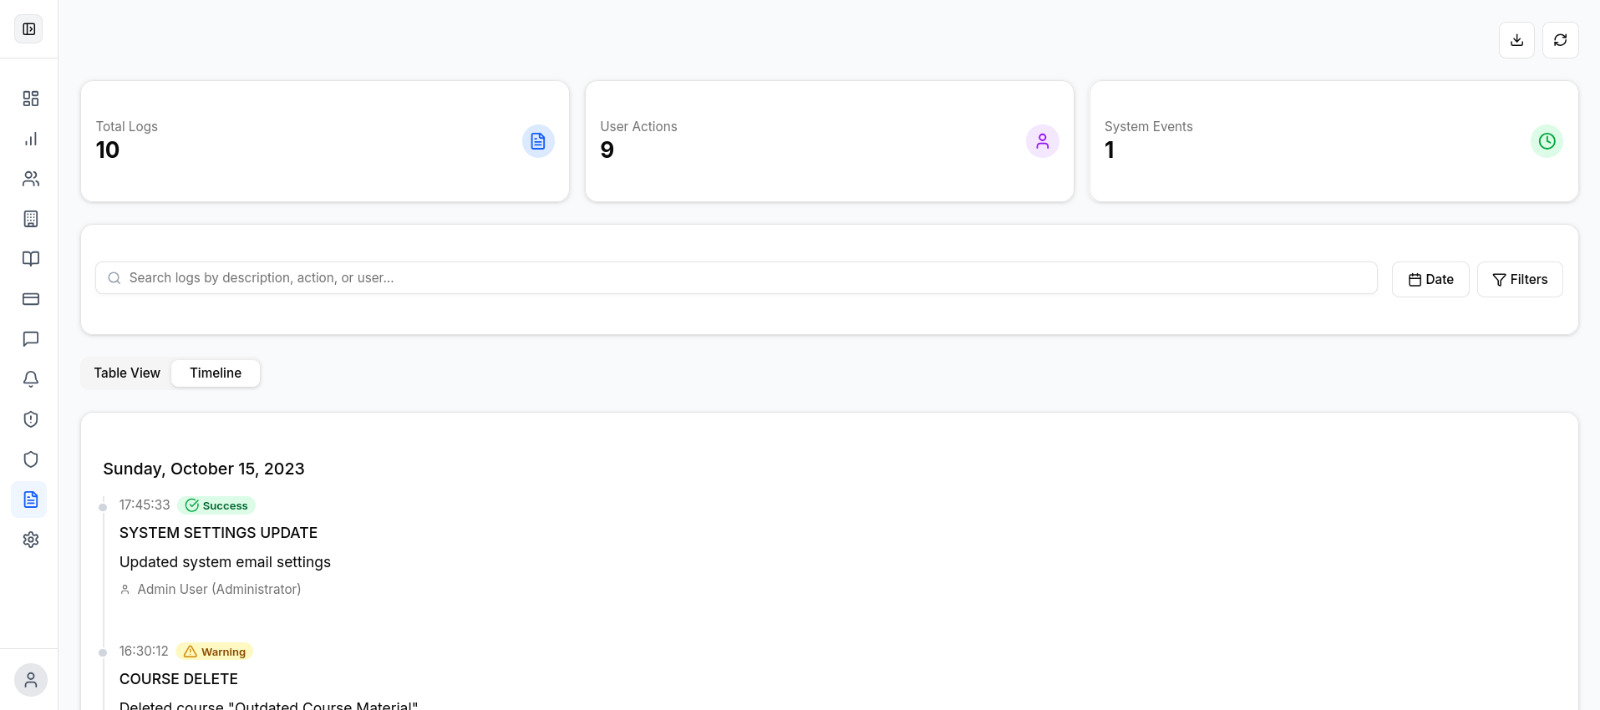
\includegraphics[width=0.85\textwidth,keepaspectratio]{old-reports/week_4_img/audit.jpeg}
  \caption{\textbf{Interface d'audit et de journalisation} pour la surveillance des activités.}
  \label{fig:audit_logs}
\end{figure}

\subsubsection{Processus de création de compte multi-étapes}

Un processus d'inscription en plusieurs étapes a été développé pour guider l'utilisateur tout en garantissant la sécurité :

\begin{itemize}
  \item \textbf{Étape 1 - Informations de base :} Collecte du nom complet et de l'adresse email
  \item \textbf{Étape 2 - Configuration de sécurité :} Création et confirmation du mot de passe avec indicateur de force
  \item \textbf{Étape 3 - Vérification :} Validation de l'email par code de vérification
  \item \textbf{Étape 4 - Personnalisation :} Choix des centres d'intérêt pour personnaliser l'expérience
\end{itemize}

\begin{figure}[H]
  \centering
  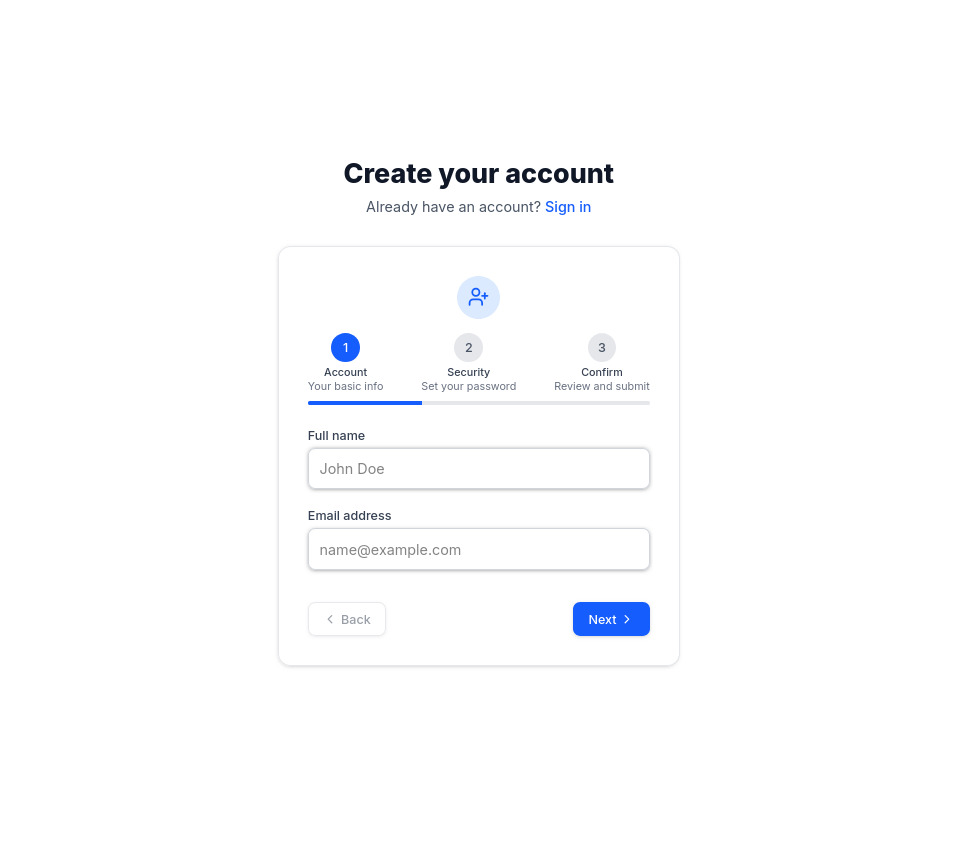
\includegraphics[width=0.4\textwidth,keepaspectratio]{old-reports/week_4_img/etap1.jpeg}
  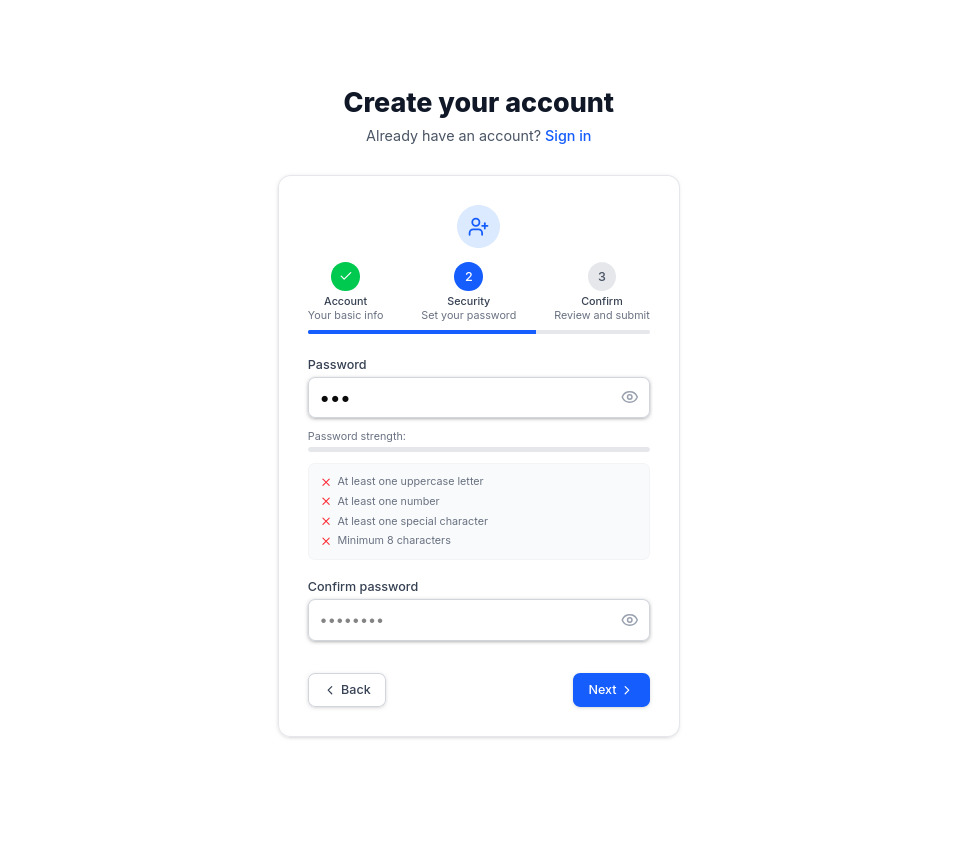
\includegraphics[width=0.4\textwidth,keepaspectratio]{old-reports/week_4_img/etap2.jpeg}
  \caption{\textbf{Étapes du processus d'inscription} - Informations de base et configuration du mot de passe.}
  \label{fig:signup_steps}
\end{figure}

\begin{figure}[H]
  \centering
  
\includegraphics[width=0.85\textwidth,keepaspectratio]{old-reports/week_4_img/sended.jpeg}
  \caption{\textbf{Email de confirmation} envoyé lors de l'inscription avec lien de vérification.}
  \label{fig:confirmation_email}
\end{figure}

Le processus inclut un système sécurisé de vérification d'email :
\begin{itemize}
  \item \textbf{Génération de tokens JWT :} Création de tokens sécurisés à durée limitée pour la vérification
  \item \textbf{Modèles d'emails personnalisés :} Emails HTML responsive avec identité visuelle de la plateforme
  \item \textbf{Suivi des statuts :} Monitoring des emails envoyés et des confirmations reçues
  \item \textbf{Relances automatiques :} Envoi de rappels après un délai si l'email n'est pas vérifié
  \item \textbf{Mécanismes anti-abus :} Limitation du nombre d'envois pour prévenir le spam
\end{itemize}

\subsubsection{Notifications et communications}

Un système de notifications avancé a été implémenté pour maintenir les utilisateurs informés :

\begin{itemize}
  \item \textbf{Centre de notifications :} Interface centralisée pour toutes les alertes et communications
  \item \textbf{Catégorisation :} Différents types de notifications (cours, système, communauté)
  \item \textbf{Personnalisation :} Options pour filtrer et ajuster les préférences de notification
  \item \textbf{État de lecture :} Distinction visuelle entre notifications lues et non lues
\end{itemize}

\begin{figure}[H]
  \centering
  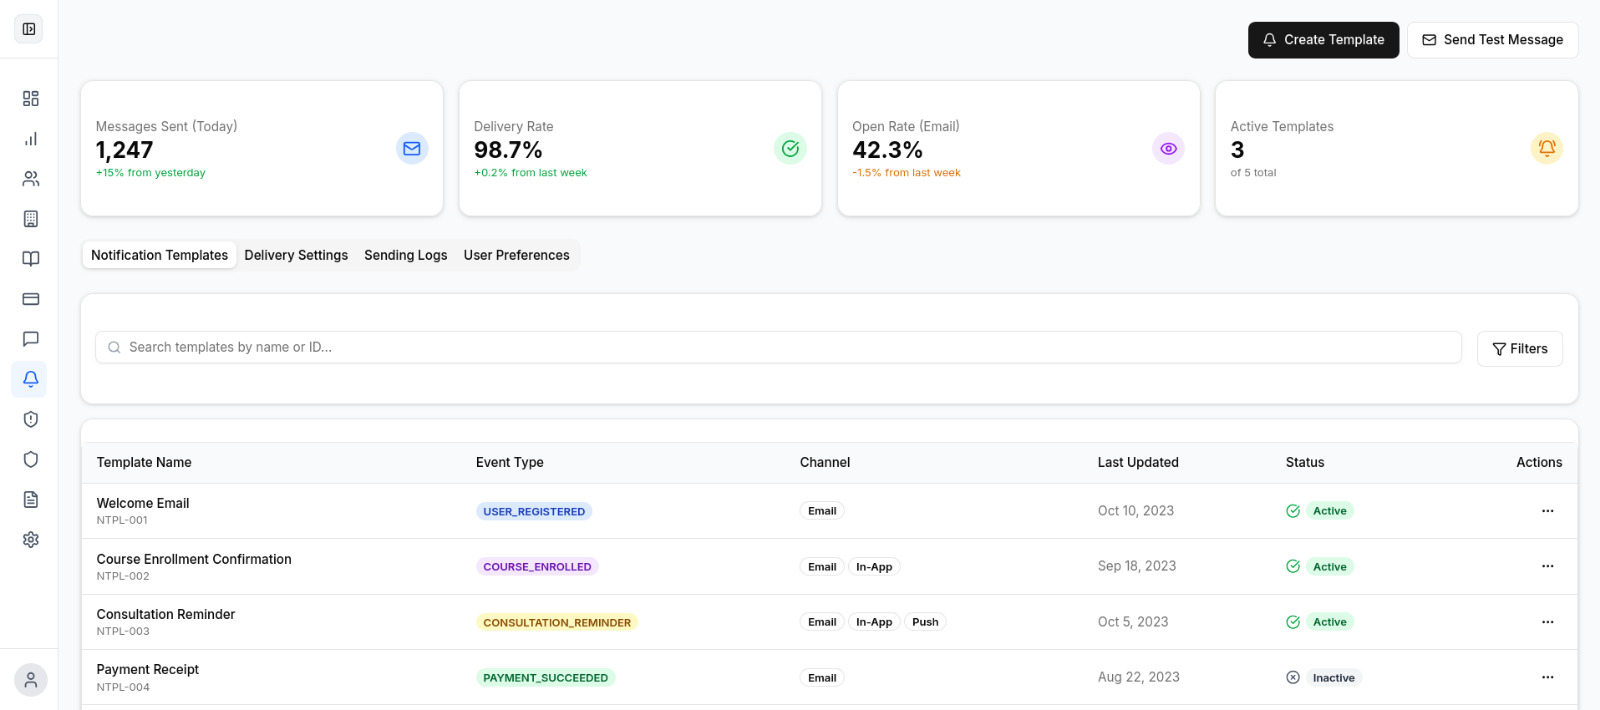
\includegraphics[width=0.85\textwidth,keepaspectratio]{old-reports/week_4_img/notifi.jpeg}
  \caption{\textbf{Centre de notifications} avec options de filtrage et de gestion.}
  \label{fig:notification_center}
\end{figure}

\subsection{Paramètres administrateur avancés}

Une interface dédiée aux paramètres administrateur a été développée pour permettre une configuration fine de la plateforme :

\begin{itemize}
  \item \textbf{Sécurité globale :} Contrôles pour les politiques de mots de passe et exigences d'authentification
  \item \textbf{Personnalisation de l'interface :} Options pour ajuster l'apparence et le comportement de la plateforme
  \item \textbf{Règles de modération :} Configuration des filtres automatiques et des seuils d'alerte
  \item \textbf{Paramètres de notification :} Gestion des communications automatiques du système
\end{itemize}

\begin{figure}[H]
  \centering
  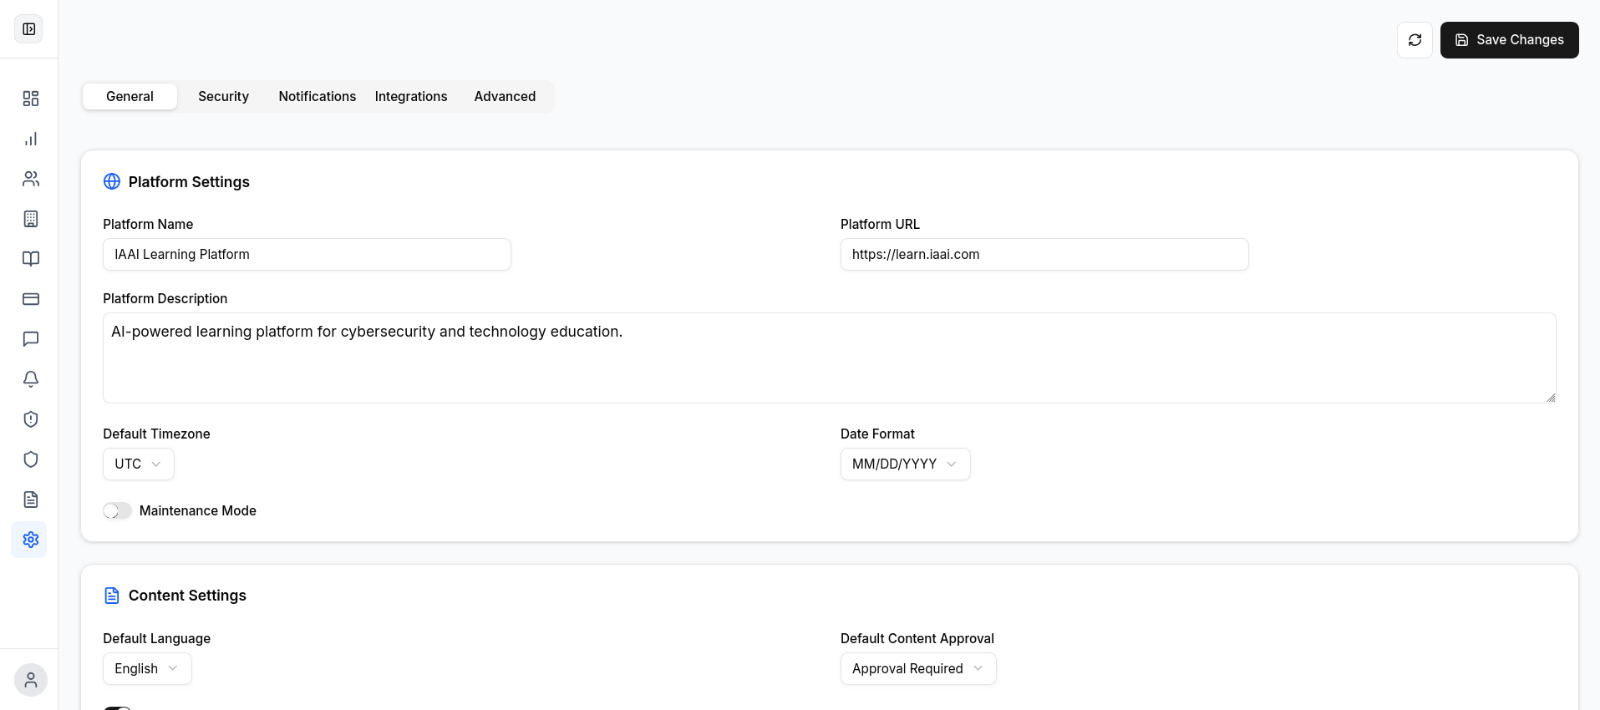
\includegraphics[width=0.85\textwidth,keepaspectratio]{old-reports/week_4_img/settings_admin.jpeg}
  \caption{\textbf{Interface des paramètres administrateur} pour la configuration de la plateforme.}
  \label{fig:admin_settings}
\end{figure}

\subsection{Parcours d'apprentissage spécialisés}

Des parcours d'apprentissage thématiques ont été développés pour couvrir différents domaines technologiques :

\begin{itemize}
  \item \textbf{Intelligence Artificielle :} Parcours couvrant les fondements de l'IA, du machine learning et du deep learning
  \item \textbf{Cybersécurité :} Formation complète sur les principes et pratiques de sécurité informatique
  \item \textbf{Compétences IT :} Parcours pour développer des compétences techniques essentielles
  \item \textbf{Préparation aux entretiens techniques :} Exercices de type LeetCode pour s'entraîner aux entretiens d'embauche
\end{itemize}

\begin{figure}[H]
  \centering
  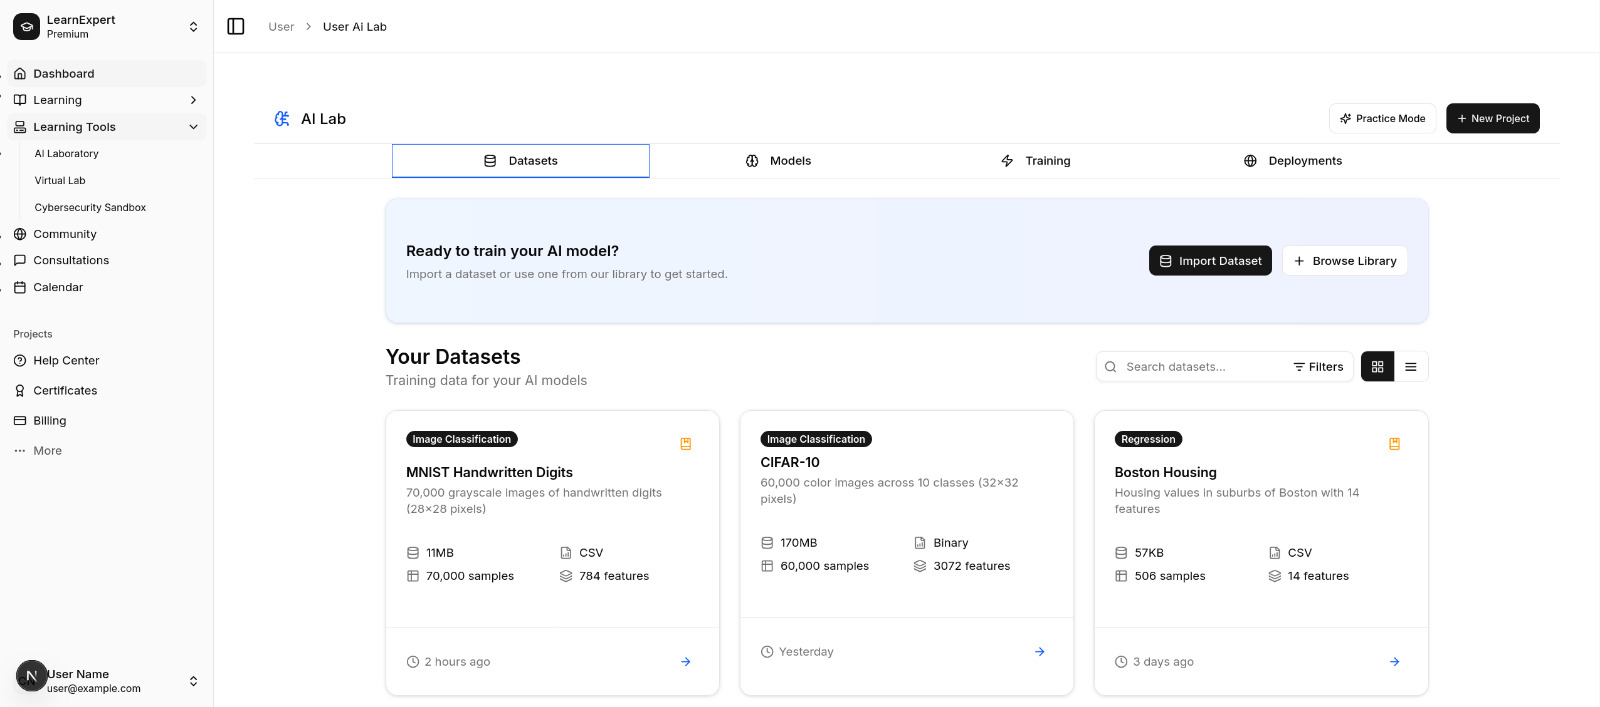
\includegraphics[width=0.4\textwidth,keepaspectratio]{old-reports/week_4_img/ai_1.jpeg}
  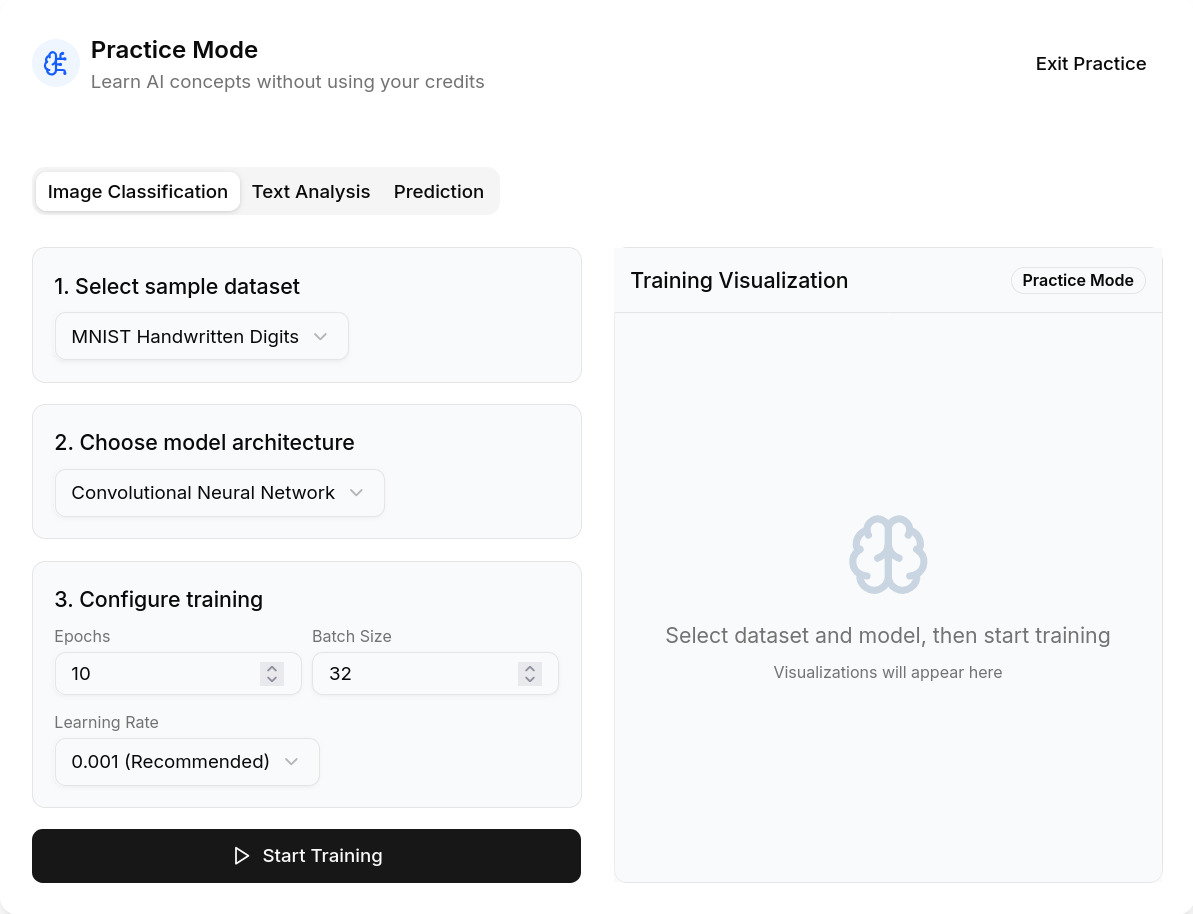
\includegraphics[width=0.4\textwidth,keepaspectratio]{old-reports/week_4_img/ai_2.jpeg}
  \caption{\textbf{Parcours d'apprentissage en Intelligence Artificielle} avec progression structurée.}
  \label{fig:ai_learning_path}
\end{figure}

\begin{figure}[H]
  \centering
  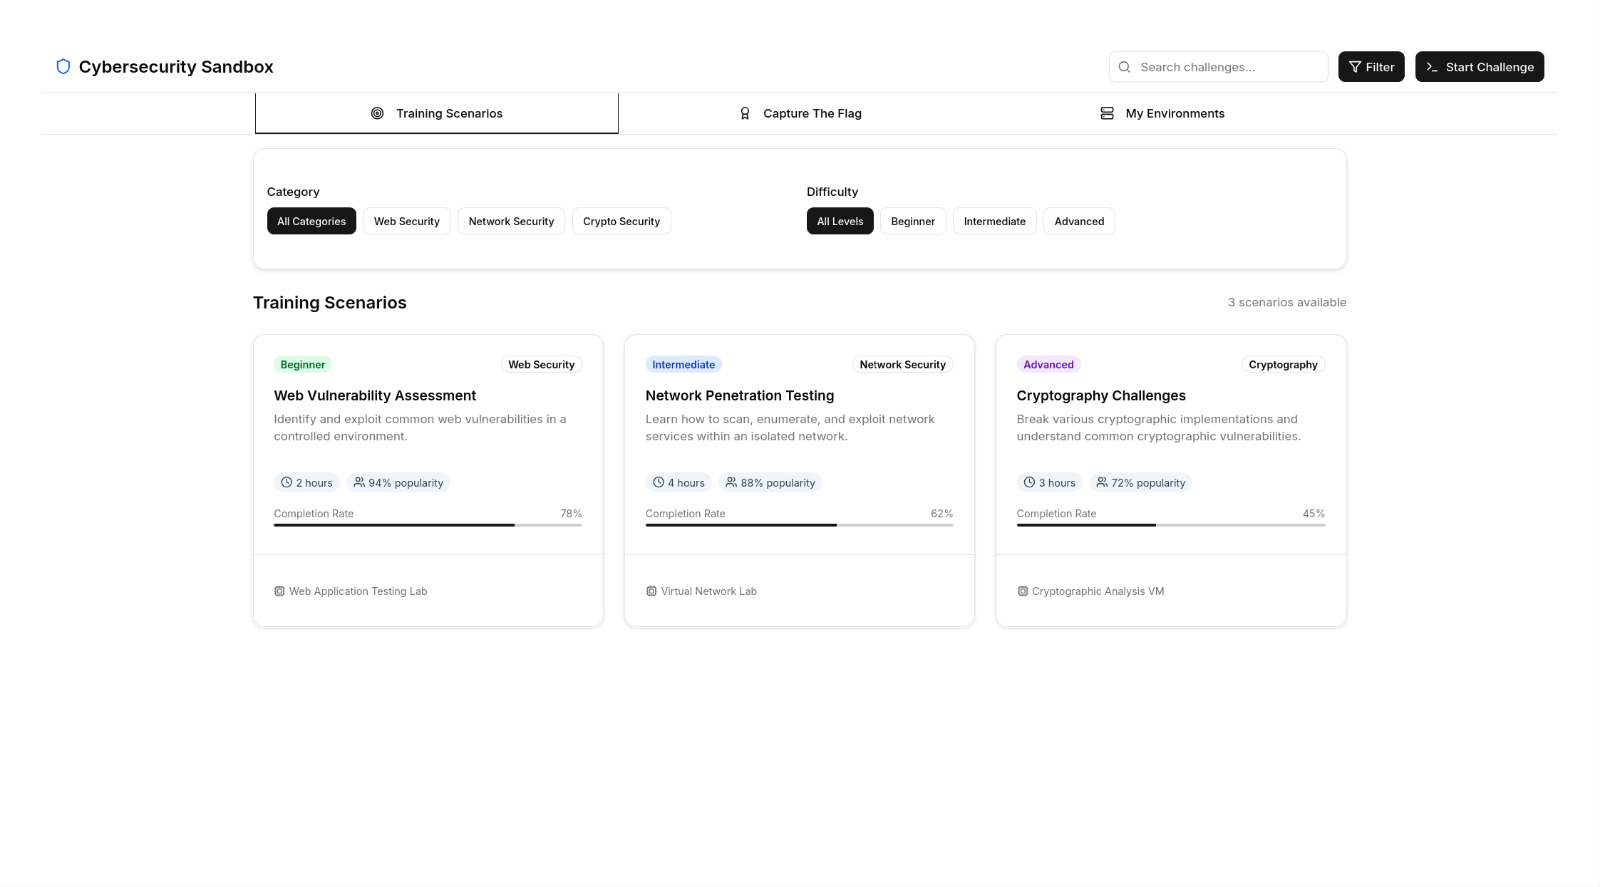
\includegraphics[width=0.4\textwidth,keepaspectratio]{old-reports/week_4_img/syber.jpeg}
  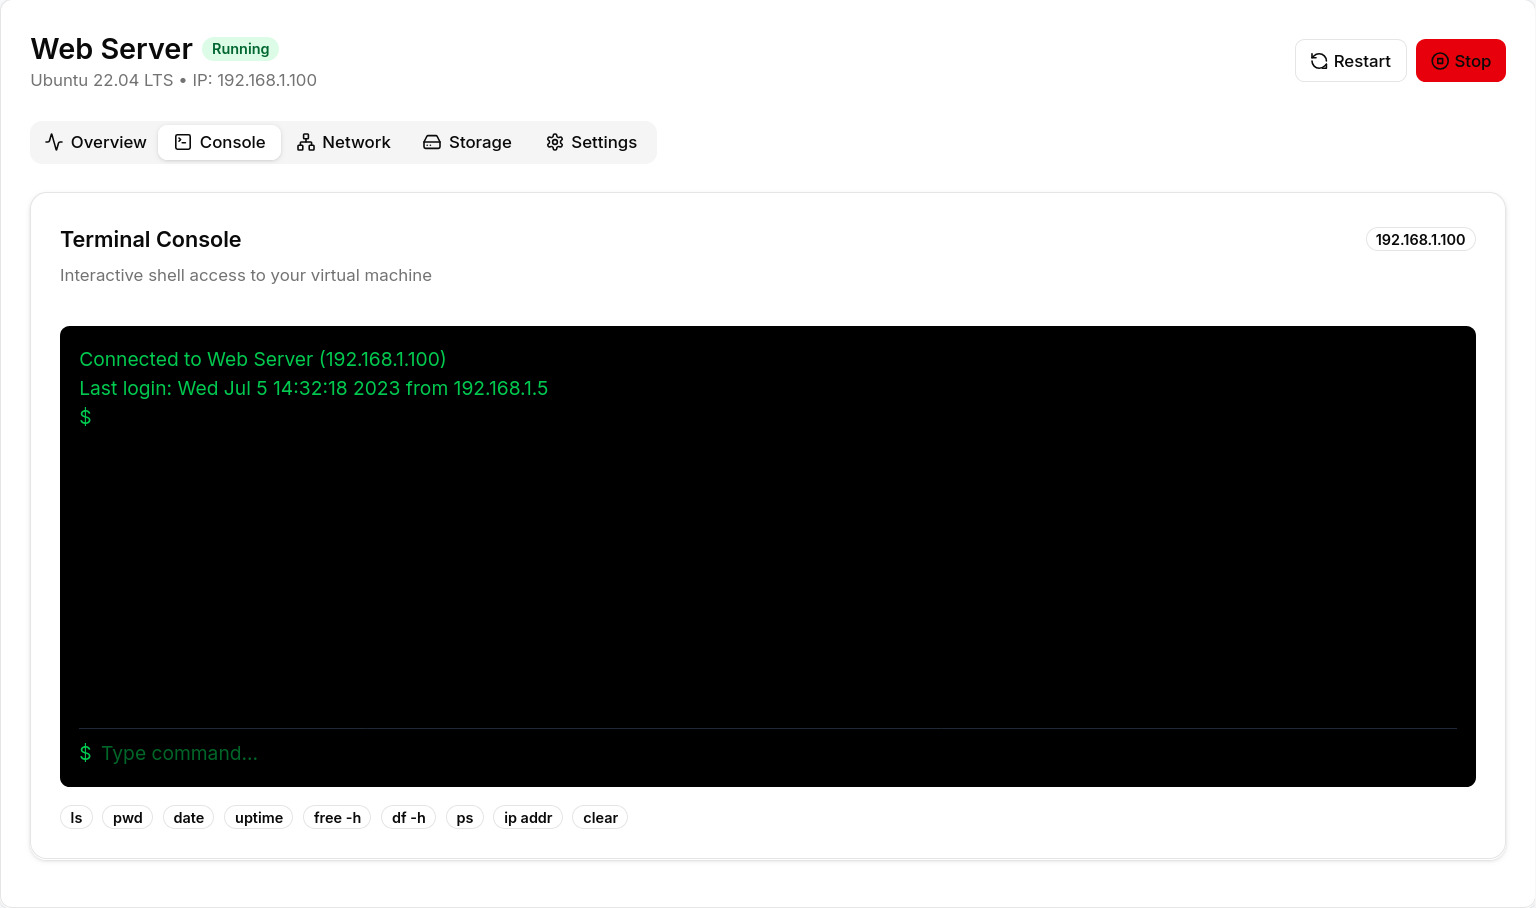
\includegraphics[width=0.4\textwidth,keepaspectratio]{old-reports/week_4_img/it.jpeg}
  \caption{\textbf{Parcours en Cybersécurité et Compétences IT} adaptés aux besoins du marché.}
  \label{fig:specialized_paths}
\end{figure}

\begin{figure}[H]
  \centering
  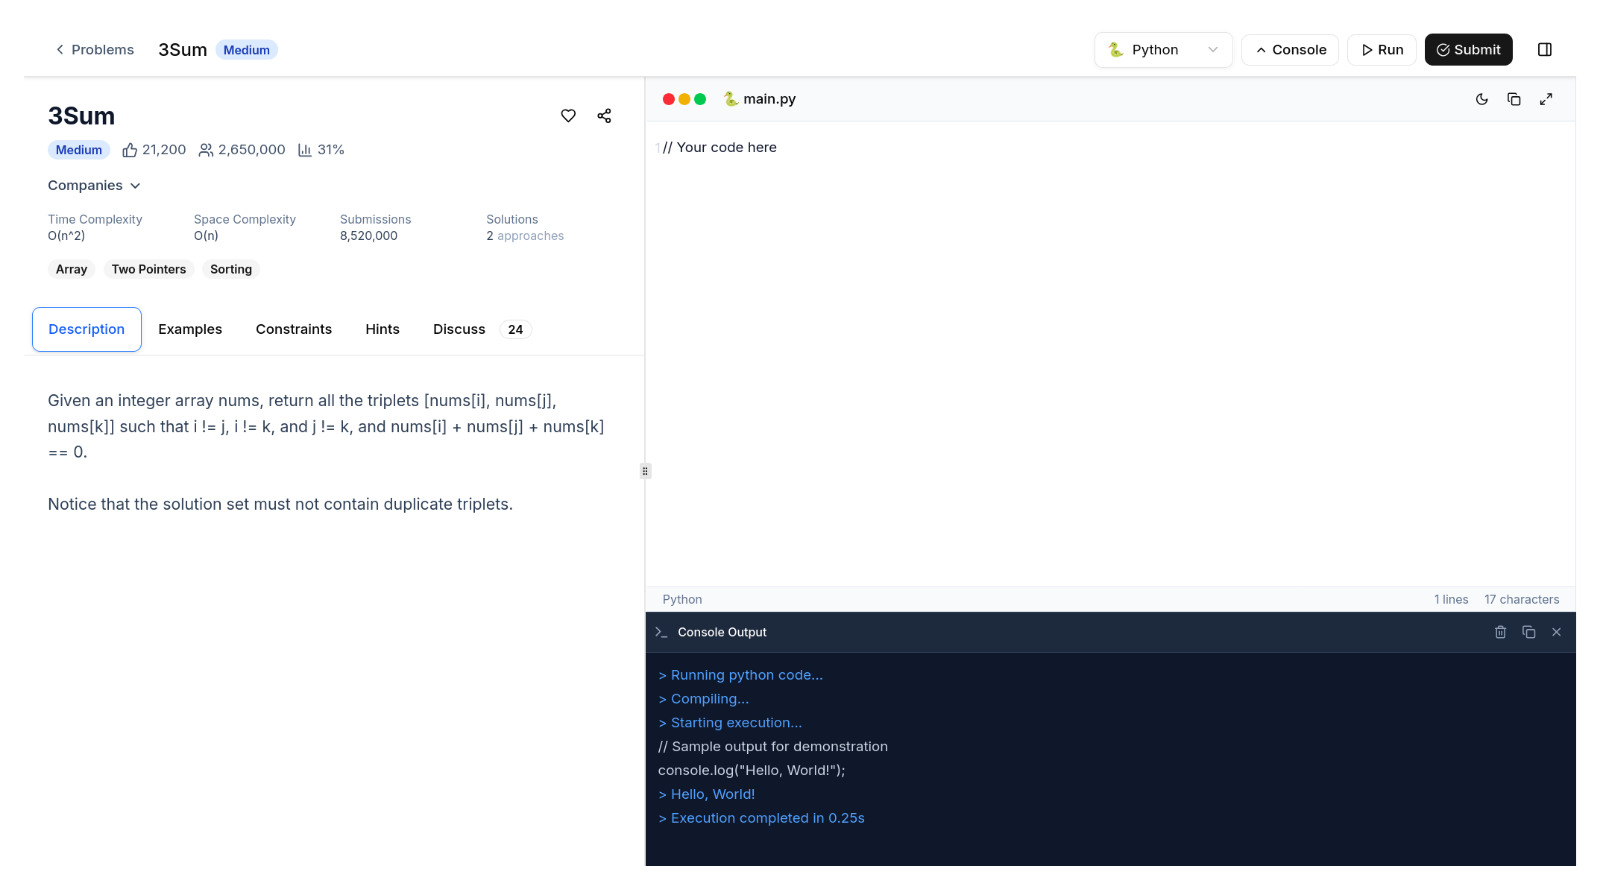
\includegraphics[width=0.85\textwidth,keepaspectratio]{old-reports/week_4_img/leetcode.jpeg}
  \caption{\textbf{Interface d'entraînement aux entretiens techniques} inspirée de LeetCode.}
  \label{fig:interview_prep}
\end{figure}

\subsection{Interfaces créateur de contenu}

Des outils spécifiques ont été développés pour permettre aux formateurs et créateurs de contenu de publier et gérer leurs cours :

\begin{itemize}
  \item \textbf{Tableau de bord créateur :} Interface dédiée avec statistiques sur les cours publiés et l'engagement des apprenants
  \item \textbf{Création de cours :} Éditeur intuitif pour structurer et publier du contenu éducatif
  \item \textbf{Gestion des cours existants :} Outils pour modifier, mettre à jour et organiser les cours publiés
  \item \textbf{Consultation et services :} Interface pour gérer les sessions de mentorat et d'assistance
\end{itemize}

\begin{figure}[H]
  \centering
  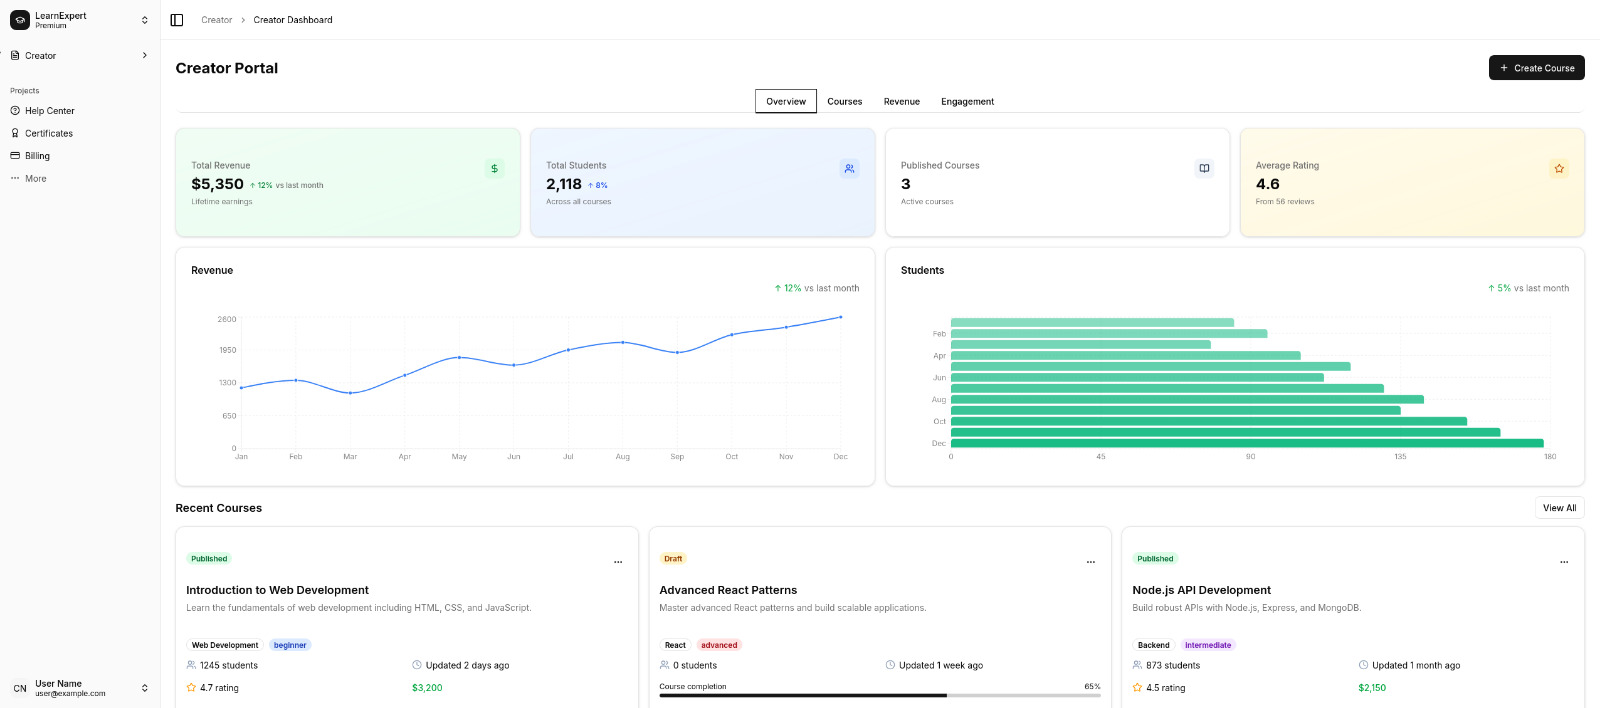
\includegraphics[width=0.85\textwidth,keepaspectratio]{old-reports/week_4_img/cdash.jpeg}
  \caption{\textbf{Tableau de bord créateur} avec statistiques d'engagement et de performance.}
  \label{fig:creator_dashboard}
\end{figure}

\begin{figure}[H]
  \centering
  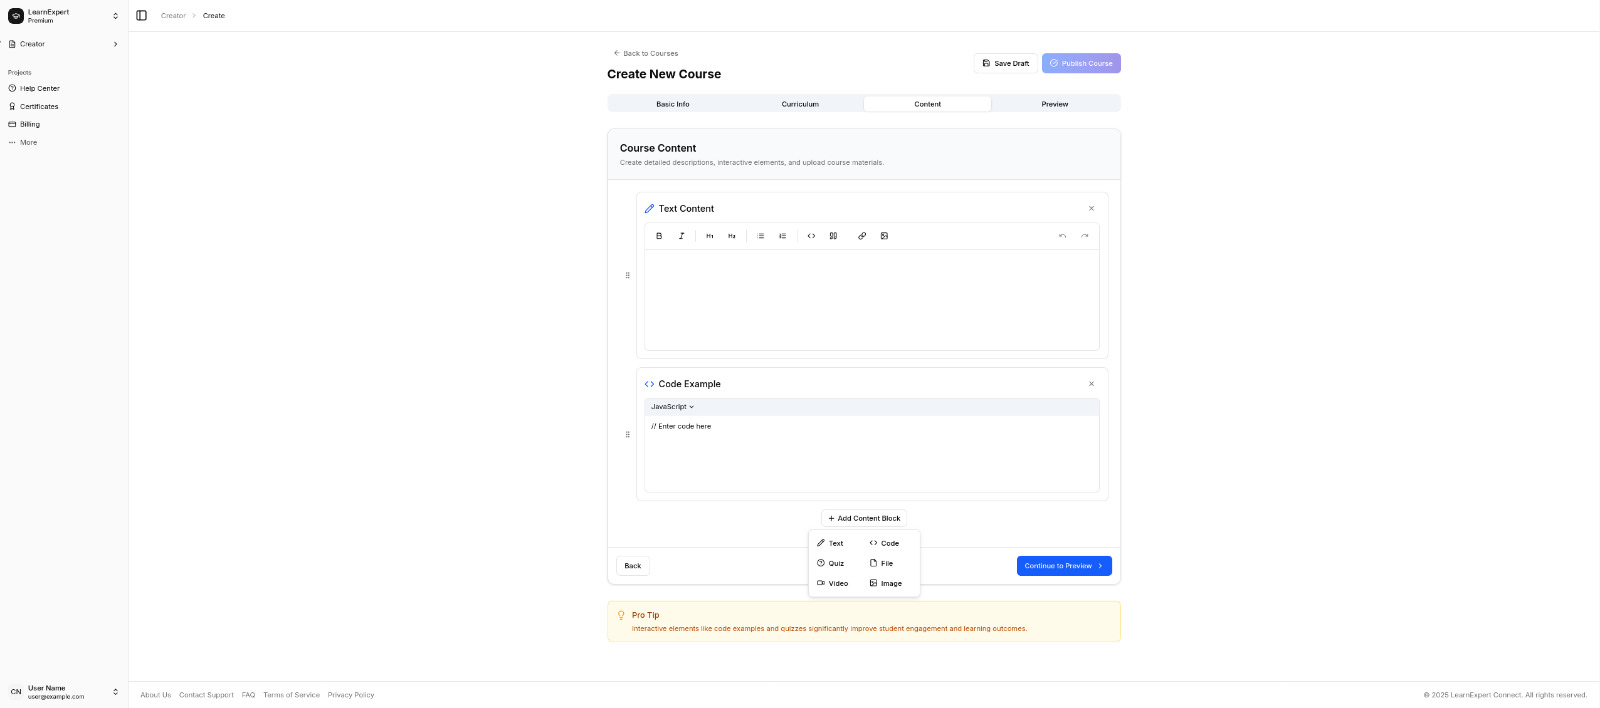
\includegraphics[width=0.85\textwidth,keepaspectratio]{old-reports/week_4_img/create_course.jpeg}
  \caption{\textbf{Interface de création de cours} avec éditeur de contenu intuitif.}
  \label{fig:course_creator}
\end{figure}

\begin{figure}[H]
  \centering
  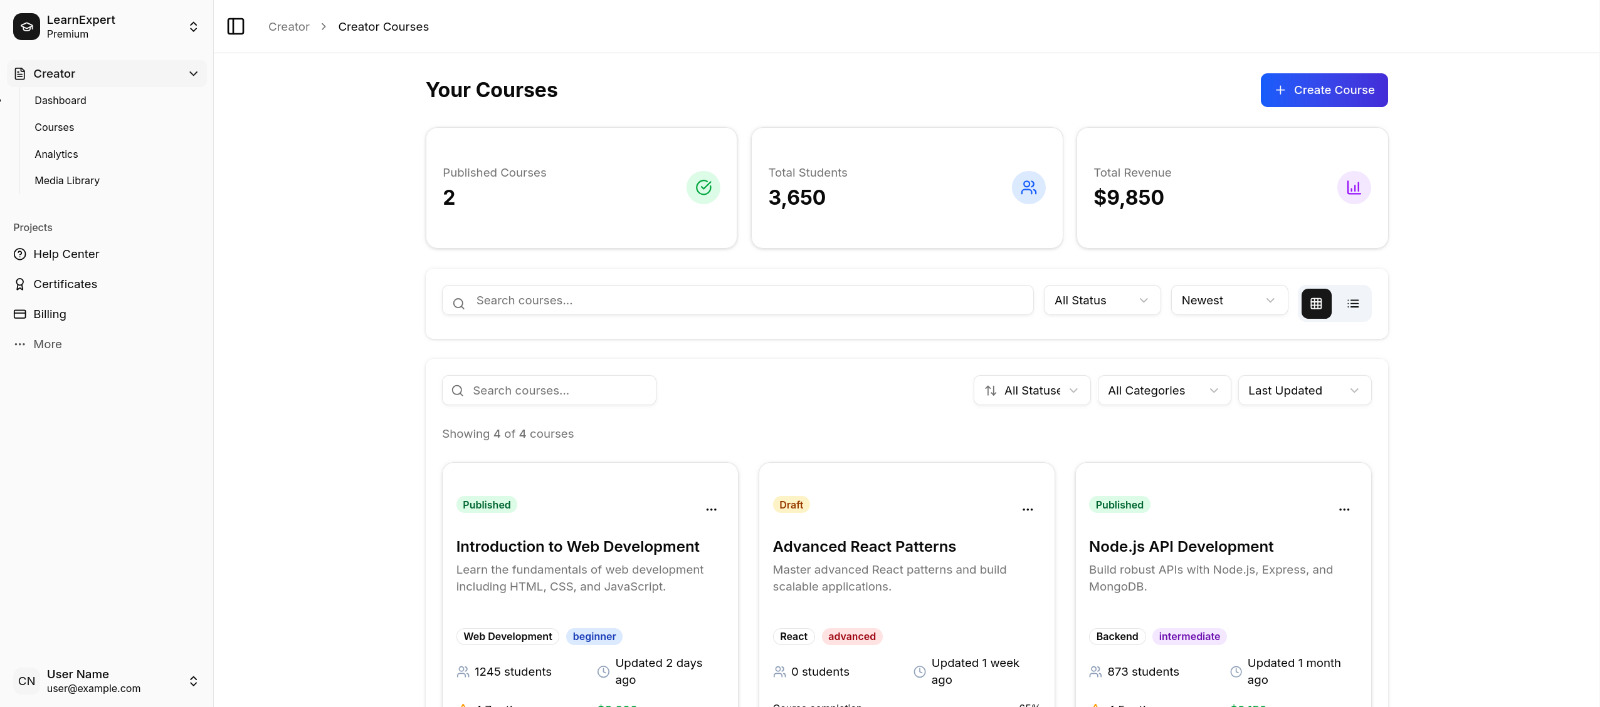
\includegraphics[width=0.85\textwidth,keepaspectratio]{old-reports/week_4_img/your_courses.jpeg}
  \caption{\textbf{Gestion des cours publiés} avec options d'édition et de suivi.}
  \label{fig:courses_management}
\end{figure}

\begin{figure}[H]
  \centering
  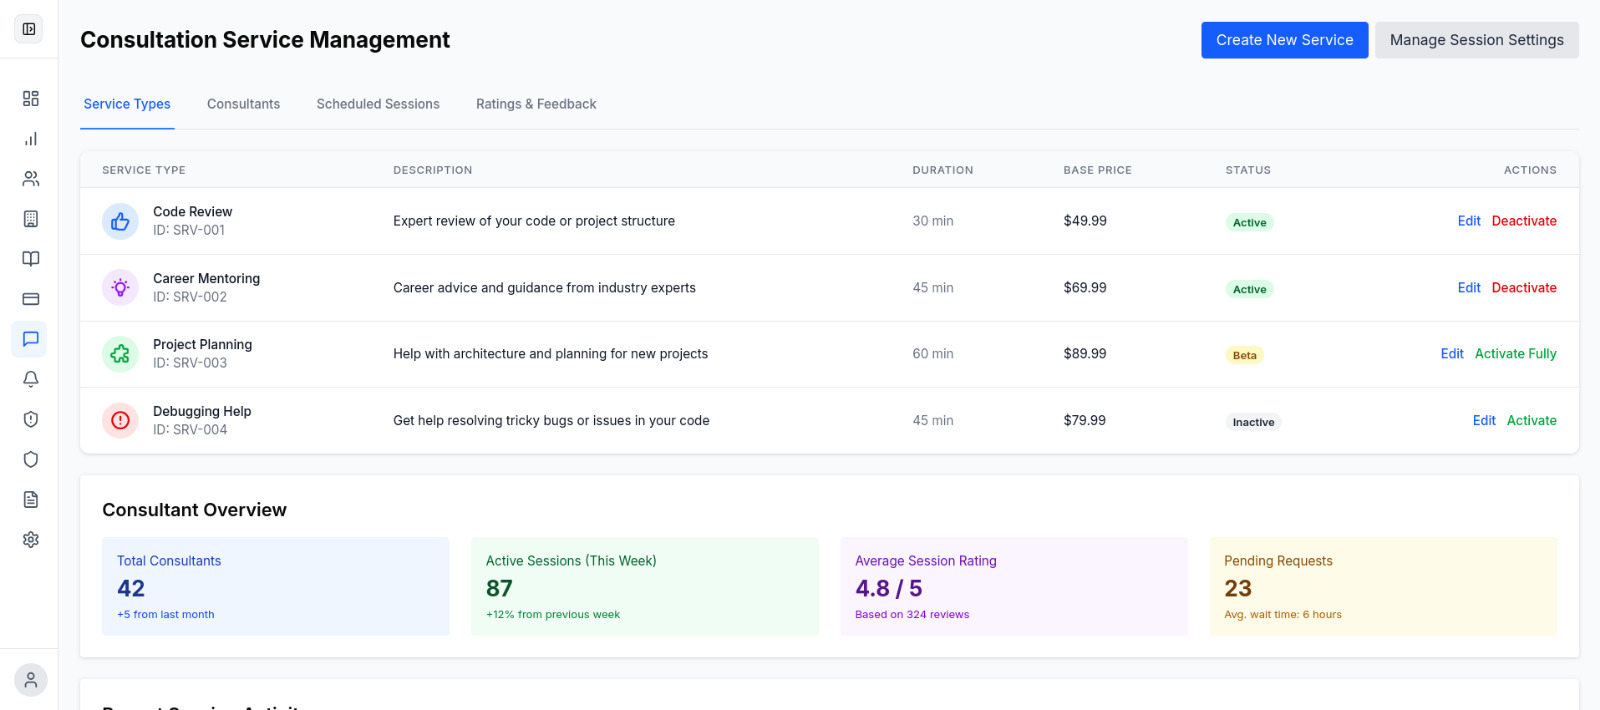
\includegraphics[width=0.85\textwidth,keepaspectratio]{old-reports/week_4_img/consultingmana.jpeg}
  \caption{\textbf{Interface de gestion des consultations} pour les mentors et experts.}
  \label{fig:consulting_management}
\end{figure}

\section{Implémentation du backend et traitement des données}

Le développement backend a été axé sur la création d'une architecture microservices robuste et la mise en place d'un système avancé de traitement des données de contenu.

\subsection{Architecture microservices}

Conformément à la conception initiale, l'architecture backend a été implémentée selon une approche microservices, avec plusieurs services spécialisés :

\begin{itemize}
  \item \textbf{Service d'authentification :} Gestion des utilisateurs, connexions et autorisations avec Supabase
  \item \textbf{Service de contenu :} Gestion et distribution des contenus de cours
  \item \textbf{Service de progression :} Suivi de l'avancement des utilisateurs
  \item \textbf{Service d'analytique :} Collecte et analyse des données d'utilisation
\end{itemize}

\begin{figure}[H]
  \centering
  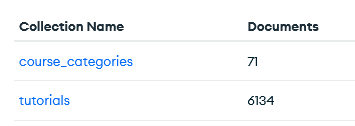
\includegraphics[width=0.9\textwidth,keepaspectratio]{week_3_img/Screenshot 2025-05-19 234047.png}
  \caption{\textbf{Organisation des données dans MongoDB Atlas} avec les différentes collections.}
  \label{fig:mongodb}
\end{figure}

\subsubsection{API Gateway avec Nginx}

Un aspect central de l'architecture microservices a été la mise en place d'Nginx comme API Gateway :

\begin{itemize}
  \item \textbf{Routage intelligent :} Redirection des requêtes vers les services appropriés
  \item \textbf{Équilibrage de charge :} Distribution efficace du trafic entre les instances de services
  \item \textbf{Mise en cache :} Optimisation des performances pour les requêtes fréquentes
  \item \textbf{Gestion des certificats SSL :} Sécurisation des communications via HTTPS
\end{itemize}

\subsubsection{Implémentation avancée de l'API Gateway}

La configuration de Nginx en tant qu'API Gateway a été optimisée pour répondre aux besoins spécifiques de la plateforme :

\begin{itemize}
  \item \textbf{Configuration de la terminaison SSL :} Mise en place de la terminaison SSL pour gérer le chiffrement/déchiffrement au niveau du gateway, soulageant les services backend
  \item \textbf{Limitation du débit :} Implémentation de limiteurs de taux de requêtes pour prévenir les abus et les attaques par déni de service
  \item \textbf{Filtrage par adresse IP :} Configuration de listes blanches et noires pour contrôler l'accès selon l'origine des requêtes
  \item \textbf{Compression des réponses :} Activation de la compression gzip pour réduire la taille des données transmises
  \item \textbf{Journalisation personnalisée :} Mise en place de formats de logs spécifiques pour faciliter l'analyse du trafic
\end{itemize}

La configuration a été structurée en plusieurs fichiers pour faciliter la maintenance :
\begin{itemize}
  \item \textbf{nginx.conf :} Configuration principale avec les paramètres globaux
  \item \textbf{conf.d/api\_gateway.conf :} Définition des routes et des règles de proxy pour chaque service
  \item \textbf{conf.d/ssl.conf :} Configuration des certificats et des paramètres de sécurité
  \item \textbf{conf.d/rate\_limiting.conf :} Règles de limitation du débit par service et par route
\end{itemize}

Cette approche modulaire permet une gestion plus flexible et évolutive, facilitant l'ajout de nouveaux services ou la modification des règles existantes sans impacter l'ensemble du système.

\subsubsection{Système d'authentification avancé}

Le service d'authentification a été développé avec une structure sophistiquée :

\begin{itemize}
  \item \textbf{Gestion des utilisateurs :} Inscriptions, connexions et gestion des profils
  \item \textbf{Système de rôles et permissions :} Contrôle d'accès granulaire avec quatre niveaux (utilisateur, créateur, consultant, administrateur)
  \item \textbf{Sécurité des données :} Politiques de sécurité au niveau des lignes (Row Level Security) pour protéger les informations sensibles
  \item \textbf{Gestion des sessions :} Suivi et sécurisation des sessions utilisateurs
  \item \textbf{API RESTful :} Endpoints documentés pour l'intégration avec le frontend
\end{itemize}

\subsubsection{Conteneurisation avec Docker}

Pour assurer la portabilité et la scalabilité de l'application :

\begin{itemize}
  \item \textbf{Dockerfiles optimisés :} Configuration spécifique pour chaque service
  \item \textbf{Docker Compose :} Orchestration de l'ensemble des services avec gestion des dépendances
  \item \textbf{Environnements isolés :} Séparation claire entre développement, test et production
  \item \textbf{Scripts de déploiement :} Automatisation du lancement et de l'arrêt des services
\end{itemize}

\subsection{Traitement des données de contenu}

Un aspect crucial du développement a été le traitement et la structuration des données de contenu éducatif. Plusieurs défis ont été rencontrés et résolus :

\begin{itemize}
  \item \textbf{Collecte et nettoyage des données :} Web scraping et normalisation des données brutes
  \item \textbf{Distinction contenu/code :} Séparation intelligente du contenu textuel et des exemples de code
  \item \textbf{Structuration cohérente :} Organisation des données dans un format adapté à l'affichage
  \item \textbf{Préservation du formatage :} Maintien des éléments de mise en forme spécifiques
\end{itemize}

\subsubsection{Défis du nettoyage des données}

La distinction entre le contenu explicatif et les extraits de code a représenté un défi majeur :

\begin{itemize}
  \item \textbf{Approches algorithmiques :} Les méthodes basées sur des expressions régulières et des heuristiques ont été testées mais n'ont atteint qu'une précision maximale de 80\%
  \item \textbf{Diversité des contenus :} La nature hétérogène des cours et la multiplicité des syntaxes de programmation ont complexifié l'automatisation
  \item \textbf{Besoin de précision :} Une séparation précise était essentielle pour l'affichage correct dans l'interface utilisateur
  \item \textbf{Volume de données :} Le traitement manuel de plus de 70 cours avec de nombreuses sections n'était pas viable
\end{itemize}

\subsection{Pipeline de traitement LLM}

Pour surmonter les défis de traitement des données, un pipeline basé sur des modèles de langage large (LLM) a été implémenté :

\begin{figure}[H]
  \centering
  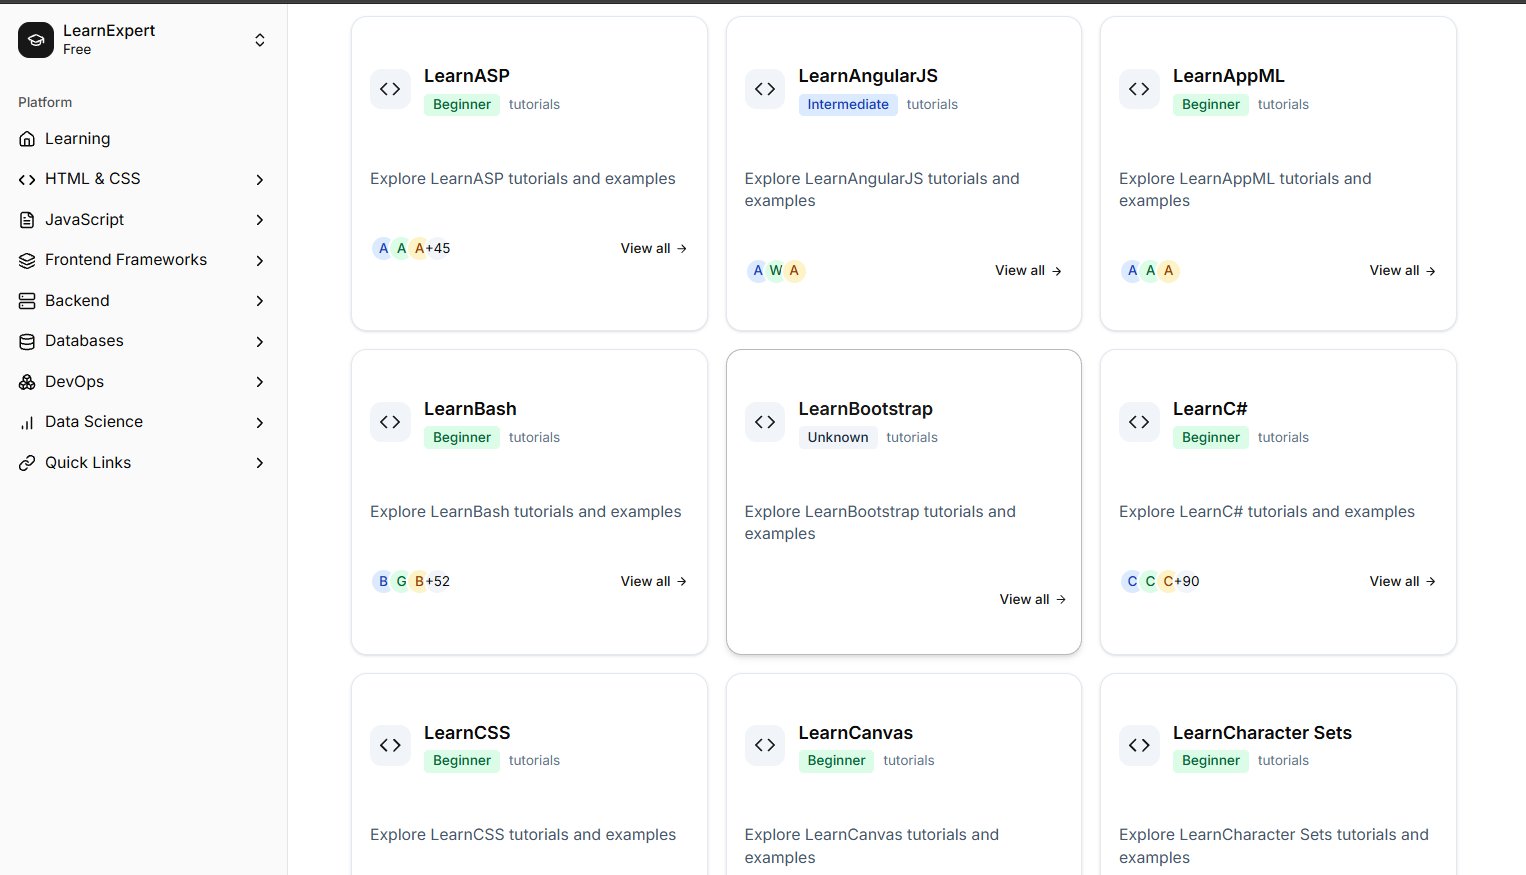
\includegraphics[width=0.9\textwidth,keepaspectratio]{week_3_img/Screenshot 2025-05-20 164411.png}
  \caption{\textbf{Interface d'administration du pipeline LLM} avec statistiques de traitement.}
  \label{fig:llm_pipeline}
\end{figure}

\subsubsection{Architecture du pipeline LLM}

Face aux limitations des approches conventionnelles, une solution innovante a été développée :

\begin{itemize}
  \item \textbf{Traitement parallèle multi-LLM :} Utilisation simultanée de plusieurs fournisseurs d'API LLM pour répartir la charge
  \item \textbf{Traitement asynchrone :} Requêtes non bloquantes permettant d'optimiser la latence globale
  \item \textbf{Segmentation intelligente :} Division des données en unités de traitement optimales pour chaque modèle
  \item \textbf{Gestion efficace des requêtes :} Assignation statique de segments aux modèles appropriés pour simplifier la gestion de la concurrence
\end{itemize}

\subsubsection{Optimisation des performances}

L'approche initiale avec un seul LLM présentait des limitations importantes en termes de temps de traitement (environ 15 heures). Des optimisations ont donc été mises en place :

\begin{itemize}
  \item \textbf{Distribution de la charge :} Répartition du traitement entre plusieurs API LLM
  \item \textbf{Réduction du temps de traitement :} Le temps total a été réduit de 15 heures à environ 7-8 heures
  \item \textbf{Amélioration de la résilience :} Tolérance aux pannes grâce à la diversification des fournisseurs
  \item \textbf{Monitoring en temps réel :} Interface d'administration pour suivre l'avancement du traitement
\end{itemize}

Cette approche innovante a permis d'atteindre une précision proche de 100\% dans la séparation du contenu et du code, tout en maintenant un temps de traitement raisonnable.

\subsection{Intégration frontend-backend}

L'intégration entre le frontend et le backend a été réalisée via des API RESTful, avec une attention particulière portée à :

\begin{itemize}
  \item \textbf{Développement de routes d'API :} Création d'endpoints pour toutes les fonctionnalités requises
  \item \textbf{Optimisation des requêtes :} Utilisation d'index et de projections pour des performances optimales
  \item \textbf{Gestion du cache :} Mise en place de stratégies de cache pour les données fréquemment consultées
  \item \textbf{Pagination :} Implémentation de mécanismes de pagination pour les listes volumineuses
\end{itemize}

\section{Fonctionnalités interactives d'apprentissage}

Un aspect distinctif de la plateforme LearnExpert est l'intégration de fonctionnalités interactives avancées pour l'apprentissage de la programmation.

\subsection{Éditeur de code interactif}

L'un des composants clés développés est l'éditeur de code interactif, basé sur Monaco Editor (la technologie derrière VS Code), offrant une expérience de codage immersive :

\begin{itemize}
  \item \textbf{Coloration syntaxique :} Support pour multiple langages de programmation (JavaScript, Python, HTML, CSS, etc.)
  \item \textbf{Exécution en temps réel :} Possibilité de tester le code directement dans l'interface
  \item \textbf{Visualisation des résultats :} Affichage immédiat du résultat pour HTML/CSS
  \item \textbf{Mode plein écran :} Option d'agrandissement pour une meilleure concentration
  \item \textbf{Thèmes personnalisables :} Choix entre différents thèmes d'édition (clair, sombre, etc.)
  \item \textbf{Dispositions flexibles :} Options pour changer la mise en page (verticale, horizontale, partagée)
  \item \textbf{Fonctionnalités d'aide :} Copie du code, réinitialisation et sauvegarde
\end{itemize}

L'implémentation technique repose sur un composant React sophistiqué qui gère l'édition de code, la prévisualisation et l'interaction avec l'utilisateur de manière fluide et réactive.

\subsection{Système de quiz et exercices}

Un système complet de quiz et d'exercices a été implémenté pour valider les connaissances des apprenants :

\begin{itemize}
  \item \textbf{Questions à choix multiples :} Avec validation immédiate des réponses
  \item \textbf{Exercices de code :} Challenges pratiques avec vérification automatique
  \item \textbf{Retour personnalisé :} Explications détaillées pour les réponses incorrectes
  \item \textbf{Progression adaptative :} Ajustement de la difficulté en fonction des performances
\end{itemize}

\subsection{Suivi de progression interactif}

Pour maintenir la motivation des apprenants, un système de suivi de progression interactif a été développé :

\begin{itemize}
  \item \textbf{Visualisation graphique :} Représentation visuelle de l'avancement global
  \item \textbf{Indicateurs de progression :} Affichage du pourcentage de complétion par module
  \item \textbf{Système de badges :} Récompenses virtuelles pour les accomplissements
  \item \textbf{Historique d'activité :} Journal détaillé des activités d'apprentissage
\end{itemize}

\section{Infrastructure et déploiement}

La mise en place d'une infrastructure solide a été une étape cruciale pour assurer la robustesse et la scalabilité de la plateforme.

\subsection{Configuration de Nginx et Docker}

Pour faciliter le déploiement et la gestion des services, une configuration avancée a été mise en place :

\begin{itemize}
  \item \textbf{Nginx comme reverse proxy :} Configuration pour gérer efficacement les requêtes entrantes et distribuer la charge
  \item \textbf{Containerisation avec Docker :} Création de Dockerfiles optimisés pour chaque composant de l'application
  \item \textbf{Orchestration avec Docker Compose :} Configuration pour la gestion des dépendances entre services
  \item \textbf{Environnements cohérents :} Garantie de la cohérence entre développement, test et production
\end{itemize}

\subsection{Déploiement et optimisation}

Le déploiement de l'application a été réalisé avec une attention particulière aux performances et à la sécurité :

\begin{itemize}
  \item \textbf{Déploiement sur Vercel :} Utilisation de la plateforme Vercel pour le déploiement du frontend Next.js
  \item \textbf{Configuration des services backend :} Déploiement des microservices avec Docker sur un serveur dédié
  \item \textbf{Optimisation des performances :} Mise en place de stratégies de mise en cache et de compression
  \item \textbf{Configuration de la sécurité :} Implémentation de HTTPS et sécurisation des API
\end{itemize}

\section{Tests et assurance qualité}

Pour garantir la fiabilité et la robustesse de la plateforme, plusieurs types de tests ont été mis en place tout au long du développement.

\subsection{Tests unitaires et d'intégration}

Des tests automatisés ont été implémentés pour vérifier le bon fonctionnement des composants individuels et de leur intégration :

\begin{itemize}
  \item \textbf{Tests unitaires :} Vérification du comportement isolé de chaque composant
  \item \textbf{Tests d'intégration :} Validation des interactions entre les différents modules
  \item \textbf{Tests de régression :} Détection des régressions potentielles lors des modifications
\end{itemize}

\subsection{Tests d'interface utilisateur}

L'interface utilisateur a été rigoureusement testée pour assurer une expérience optimale :

\begin{itemize}
  \item \textbf{Tests de compatibilité :} Vérification du rendu sur différents navigateurs (Chrome, Firefox, Safari, Edge)
  \item \textbf{Tests de responsive design :} Validation de l'adaptation aux différentes tailles d'écran
  \item \textbf{Tests d'accessibilité :} Conformité aux standards WCAG pour une plateforme inclusive
  \item \textbf{Tests d'utilisabilité :} Évaluation de l'intuitivité et de la fluidité de navigation
\end{itemize}

\subsection{Tests de performance}

Des tests de performance ont été conduits pour identifier et résoudre les goulots d'étranglement potentiels :

\begin{itemize}
  \item \textbf{Mesure des temps de chargement :} Analyse des performances de chargement initial
  \item \textbf{Optimisation des requêtes :} Amélioration des performances des requêtes API
  \item \textbf{Tests de charge :} Simulation d'utilisation intensive pour évaluer la robustesse
  \item \textbf{Profilage mémoire :} Identification et résolution des fuites mémoire potentielles
\end{itemize}

\section{Conclusion}

La phase de réalisation et de mise en œuvre du système a permis de transformer la vision initiale en une plateforme fonctionnelle et performante. L'utilisation de technologies modernes comme Next.js, MongoDB et les modèles LLM a permis de relever efficacement les défis techniques rencontrés.

Le développement a suivi une approche itérative, avec des améliorations continues basées sur les retours et les tests. Cette méthodologie a permis d'aboutir à une plateforme e-learning robuste, intuitive et offrant une expérience d'apprentissage immersive grâce à ses fonctionnalités interactives avancées.

L'implémentation d'une architecture microservices, combinée à un pipeline de traitement des données innovant utilisant des modèles LLM en parallèle, témoigne d'une approche technique sophistiquée visant à résoudre des problèmes complexes. Ces choix techniques ont non seulement permis d'atteindre les objectifs fonctionnels du projet, mais ont également posé les bases d'une plateforme évolutive et maintenable.

La combinaison d'une interface utilisateur soignée, d'une architecture backend performante et d'un traitement intelligent des données éducatives constitue la base solide sur laquelle la plateforme LearnExpert pourra évoluer et s'enrichir dans le futur.

